\documentclass{../content16b}

\usepackage{ccicons}
\newcommand{\unit}[1]{\ensuremath{\,\text{#1}}}
\newcommand{\Ohm}[1]{\unit{\ensuremath{\Omega}}}
\counterwithin{section}{chapter}

%% style override
\nouppercaseheads
\aliaspagestyle{title}{empty}
\pagestyle{ruled}
%% not sure if I want to hang these!!
% \chapterstyle{hangnum}
% \hangsecnum
\begin{document}
\title{EECS 16B Notes}
\author{Simon Kuang, Seth Sanders}
\date{Spring (now Fall) 2020}
\frontmatter
\maketitle

\section{Introduction}
These are notes for EECS 16B, a freshman-level survey of topics in electrical engineering. I (Simon) mostly wrote them during the \href{https://inst.eecs.berkeley.edu/~ee16b/sp20/}{Spring 2020 semester} of EECS 16B paraphrasing, Prof.~Sanders's lectures the same semester.
The words and sentences are my own; however, I owe the graphics and some editing to Seth, and a fair bit of mistake-catching to our diligent students.

If you find a mistake or can suggest an improvement, \href{https://github.com/simontheflutist/eecs16b-notes}{let me know on GitHub}.

These notes are released under \href{https://creativecommons.org/licenses/by-nc-sa/4.0/}{Creative Commons Attribution-NonCommercial-ShareAlike 4.0 International (\ccbyncsa)}.

The file you're viewing was compiled at \DTMnow.

\newpage
\tableofcontents
\newpage
\listoffigures

\mainmatter
\renewcommand{\printchaptername}{\chapnamefont Lecture}
\chapter{16A review and prerequisites}
\section{The language of circuits}
Electrical circuits are models, specifically, abstractions of underlying physics-based descriptions of realities that govern behavior of an electrical system under analysis. Mathematically, circuits are
collections of \emph{nodes} joined by \emph{branch elements}.
Between every pair of adjacent nodes there is a \emph{voltage difference},
 measured in volts,
as well as a \emph{current}, measured in amps.
You should be able to explain, both in approximate
physical terms, and, if possible,
by a mechanical analog, what voltage and current are.
Given a circuit drawing, you should be able to write a comprehensive set
of voltage-current constraints that fully predicts what is happening
in the circuit.
For a well-posed circuit model with \(N\) nodes, one preferred method is Nodal Analysis, which involves writing \(N - 1\) linearly independent KCL node equations, and incorporating KVL and element branch consraints while writing the node equations.

\begin{figure}[H]
  \begin{center}
    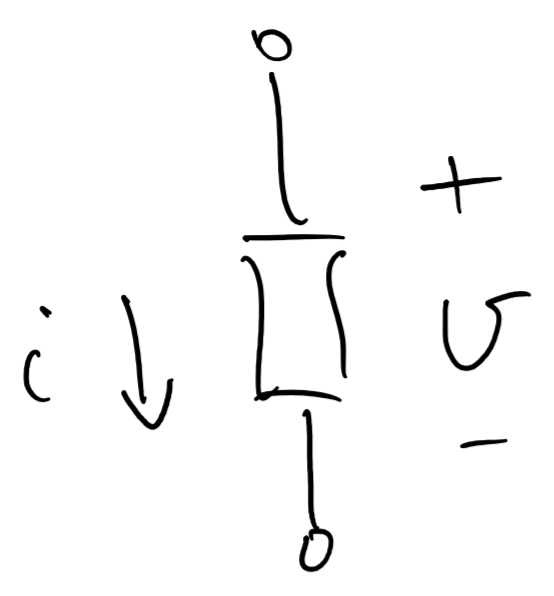
\includegraphics[width=0.25\linewidth]{figures/passive-sign}
  \end{center}
  \caption{Current and voltage annotated on a passive element.}
  \label{figure:circuit-review:passive-sign-convention}
\end{figure}
Understand how current and voltage are annotated on a circuit.
% A passive circuit element, such as a resistor, capacitor, or
% inductor\footnote{To be introduced later in 16B.}
% participates in dissipating energy from a circuit, mainly as heat.
Our terms are ``voltage \emph{across} branch element X''
and ``current \emph{through} branch element X.''
The phrases ``voltage
\emph{through}\ldots'' or ``current \emph{across}\ldots'' do not
make sense.
Understand, as shown in
Fig.~\ref{figure:circuit-review:passive-sign-convention},
that the reference directions for voltage and current are such that
% However,
% on an active circuit element, the arrow is drawn in the opposite direction.
power absorbed by a circuit element is given by
the formula \(vi\).
%\footnote{You can remember this by the Latin noun
% \emph{virtus}, which means ``strength.''}

\section{Current-voltage characteristic}
% Circuits are fully determined by their schematics because each element
% imposes a one-to-one\footnote{The assumption that
% I-V is a one-to-one correspondence
% can be relaxed in the physical world as well as in exotic exam problems,
% but only rarely.}
% constraint between its current and voltage.

\subsection{Resistor}
\begin{figure}
  \centering
  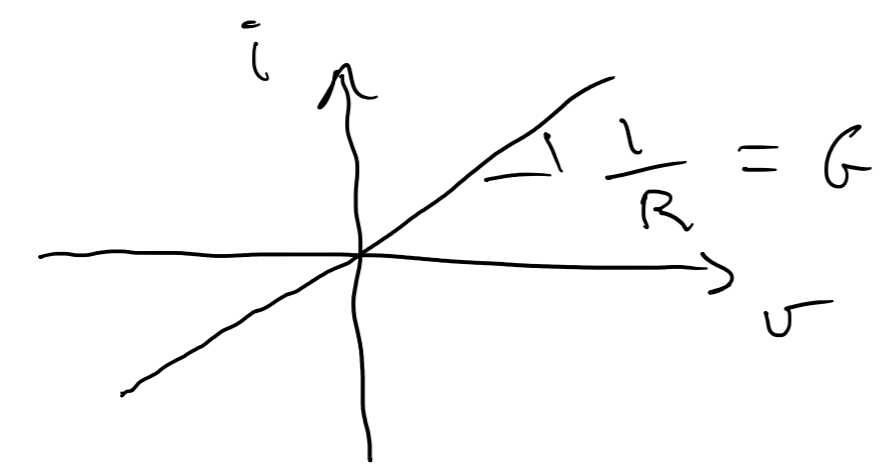
\includegraphics[width=0.5\linewidth]{figures/IV-resistor}
  \caption{I-V characteristic of a resistor.}
  \label{figure:circuit-review:IV-resistor}
\end{figure}
As shown in Fig.~\ref{figure:circuit-review:IV-resistor},
resistors enforce a proportionality relationship between
current and voltage:
\begin{align}
  V &= RI\\
  I &= GV
\end{align}
The ratio \(V/I\) is called \emph{resistance}.
The ratio \(I/V\) is called \emph{conductance}.

\subsection{Voltage source}
\begin{figure}
  \centering
  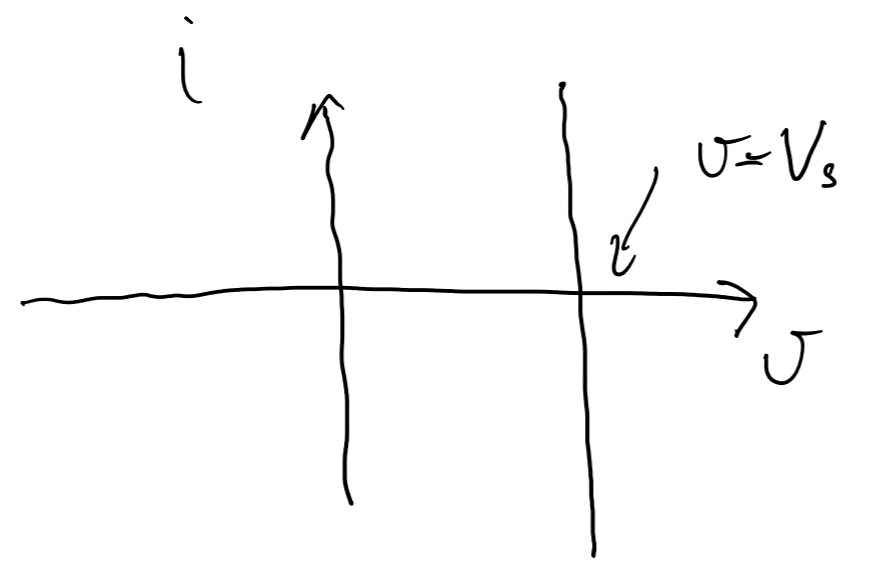
\includegraphics[width=0.5\linewidth]{figures/IV-voltage-source}
  \caption{I-V characteristic of a voltage source.}
  \label{figure:circuit-review:IV-VS}
\end{figure}
As shown in Fig.~\ref{figure:circuit-review:IV-VS},
a voltage source will provide any current (or none at all) to
maintain its target voltage.

\subsection{Current source}
\begin{figure}
  \centering
  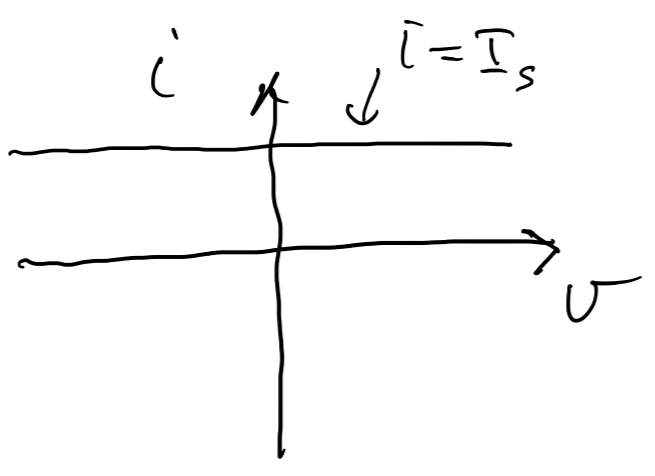
\includegraphics[width=0.4\linewidth]{figures/IV-current-source}
  \caption{I-V characteristic of a current source.}
  \label{figure:circuit-review:IV-CS}
\end{figure}
As shown in Fig.~\ref{figure:circuit-review:IV-CS},
a current source will provide any voltage (or none at all) to
maintain its target current.

\subsection{Circuit-solving techniques}
Be familiar with the following methods for solving circuits:
\begin{itemize}
  \item Series elements, e.g.~two resistors in series
  \item Parallel elements, e.g.~two resistors in parallel.
  \item Voltage and current dividers
  \item Kirchoff's voltage and current laws
  \item Norton and Th\'evenin equivalent circuits
  \item Nodal analysis
  \item Power calculations
\end{itemize}

\section{Linear algebra}
Know what a vector is. Know what eigenvalues and eigenvectors are,
and know how to solve for the eigenvalues and eigenvectors of a matrix,
by solving for the null space of \(A - \lambda I\), where
\(\lambda\) is an indeterminate. Know why this technique works.

\chapter{Transistor Circuits}


\section{\textsc{mosfet} behavior at a low level}
Transistors are nonlinear circuit elements that are integral to building digital electronics.
We'll focus on a class of transistor called \textsc{mosfet}
(\emph{metal-oxide semiconductor field-effect transistor}),
of which there are two types, \textsc{nmos} and \textsc{pmos}.
For the most part, we will view \textsc{mosfet}s from a digital perspective as voltage-controlled switches (more on that later), but we'll first have a look at the analog
% \footnote{You'll see the words ``digital'' and ``analog'' a lot. Digital devices process continuous quantities from outdoors by treating them as a collection of digits (similar to how we write numbers). Analog devices process continuous quantities by encoding them in electrical continua; for example, a site on a digital camera sensor converts light intensity to voltage (analog), and then to a digit representation (digital) for storage.}
world under the hood.

The physical makeup of a \textsc{mosfet} is shown in \autoref{figure:lec2-MOS}.
It is a device built on a silicon substrate with three terminals:
\emph{source} (S), \emph{drain} (D), and \emph{gate} (G).
What makes a transistor a transistor is
2) mediated by gate voltage. (No current enters the gate of a \textsc{mosfet}: \(I_\text{G}\) = 0.)
1) a current-voltage characteristic between drain and source,
These quantities are labeled on \autoref{figure:lec2-NMOS}.
Notice that voltages are understood with reference to their difference from \(V_\text{S}\), so:
\begin{itemize}
  \item D-S current-voltage characteristic is between \(I_\text{D}\) and \(v_\text{DS} = v_\text{D} - v_\text{S}\),%
  % \footnote{The subscript ``DS'' can be thought of as ``D minus S''
  % or ``from S to D.''}
  \item parameterized by \(v_\text{GS} = v_\text{G} - v_\text{S}\).
\end{itemize}


\subsection{The role of \(v_\text{GS}\) in \textsc{nmos}}
\begin{figure}
  \centering
  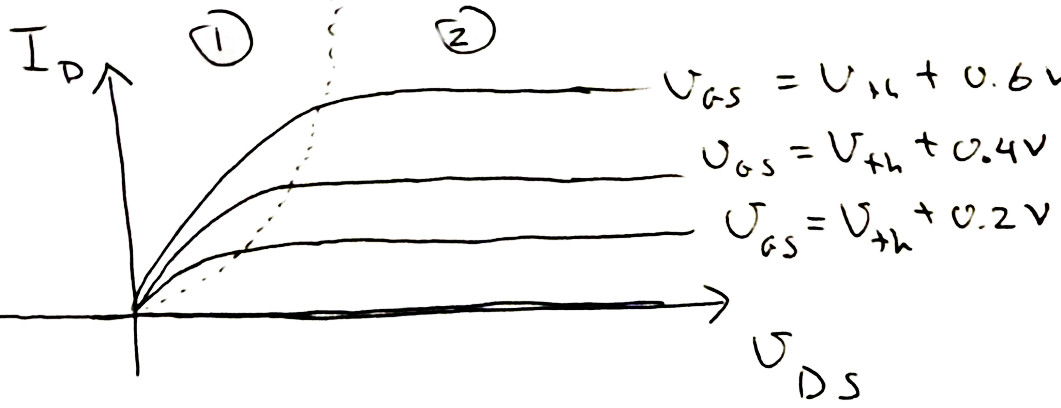
\includegraphics[width=0.8\linewidth]{figures/NMOS-IV}
  \caption{I-V characteristic of an \textsc{nmos} transistor at different values of \(v_\text{GS}\).}
  \label{figure:lec2-NMOS-IV}
\end{figure}
\autoref{figure:lec2-NMOS-IV} depicts several current-voltage characteristics of an \text{nmos}, parameterized by \(v_\text{GS}\).
There's a lot happening on this graph in both the vertical and horizontal directions.
Here's a self-guided tour:
\begin{itemize}
  \item Notice the horizontal line lying along the positive
  \(v_\text{DS}\)-axis.
  This is the plot of the I-V characteristic when
  \(v_\text{GS} < v_\text{t,n}\), where
  \(v_\text{t,n} > 0\)
  is the threshold voltage for an \textsc{nmos} transistor.
  The current-voltage characteristic is \(I=0\),
  the transistor is behaving as a current source corresponding to zero current%
  ---in other words, it's an open circuit.
  The transistor is ``off.''\,\footnote{English semantics for ``on'' and ``off'' in circuits can be counterintuitive. An open circuit/switch is off, and vice versa.}
  \item
  Notice that three I-V curves, parameterized
  by how much \(v_\text{GS}\) exceeds \(v_{t,n}\),
  lie above the line \(I = 0\).
  % \(v_\text{GS} = v_\text{t,n} + 0.2\unit{V}\),
  % \(v_\text{GS} = v_\text{t,n} + 0.4\unit{V}\),
  % and
  % \(v_\text{GS} = v_\text{t,n} + 0.4\unit{V}\).
  Each of them is intersected by what looks like the eastern half of
  a dotted upward-facing parabola rising
  from the origin.
  This parabola divides the quadrant into two regions, one left and one right.
  The left region is called region 1; the right region is called region 2.
  \item
  Focus on region 1, which is called the Linear Region.
  Notice that in region 1 near the origin, \(I_\text{D}\) and \(v_\text{DS}\) are proportional for every value of \(v_\text{GS}\).
  The slope \(G = I_{D} / v_\text{DS}\) increases for higher values of
  \(v_\text{GS}\).
  This means that the D-S resistance \(R = G^{-1}\) transitions from
  \(\infty\) to a finite (perhaps small) value as
  \(v_{GS}\) increases past \(v_{t,n}\).
  A resistor that can alternate between finite and infinite resistance
  is called a switch: in the Linear Region the transistor is a voltage-controlled switch.
  \item
  Focus on region 2, which is called Saturation,
  Here the \(I_{D}\) increases only very weakly
  as \(v_\text{DS}\) increases.%
  % \footnote{Actually this model is somewhat idealistic.
  % In fact \(I_\text{D}\) is very weakly increasing in \(v_\text{DS}\).}
  For a given \(V_{DS}\),
  \(I_\text{D}\) increases with increasing \(v_\text{GS}\):
  the transistor behaves approximately as a voltage-controlled current source!
\end{itemize}
These characteristics are summarized in \autoref{figure:lec2-NMOS-regime-table}.
Regions 0 and 1 can be used to implement a switch.
Region 2 is used for analog electronics---dependent sources,
  amplifiers, etc.

\begin{figure}
  \centering
  \begin{tabular}{lllll}
    region \# & on/off? &
    \(v_\text{GS}\) predicate & \(v_\text{DS}\) predicate
    & name\\\hline
    0 & off & \(v_\text{GS} < v_{t,n}\) & any & \\
    1 & on & \(v_\text{GS} > v_{t,n}\) & low & ``linear region''\\
    2 & on & \(v_\text{GS} > v_{t,n}\) & high & ``saturation''
  \end{tabular}
  \caption{Regions of an \textsc{nmos} I-V characteristic.}
  \label{figure:lec2-NMOS-regime-table}
\end{figure}

\subsection{\textsc{pmos} transistors: opposite of \textsc{nmos}}
\begin{figure}
  \centering
  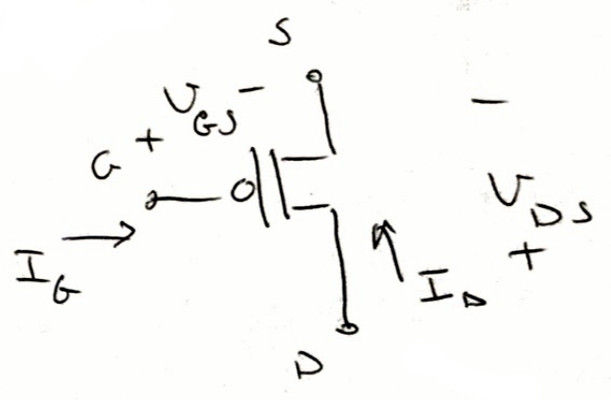
\includegraphics[width=0.5\linewidth]{figures/PMOS-currents-voltages}
  \caption{Currents and voltages labeled on a \textsc{pmos} transistor.}
  \label{figure:lec2-PMOS}
\end{figure}
\begin{figure}
  \centering
  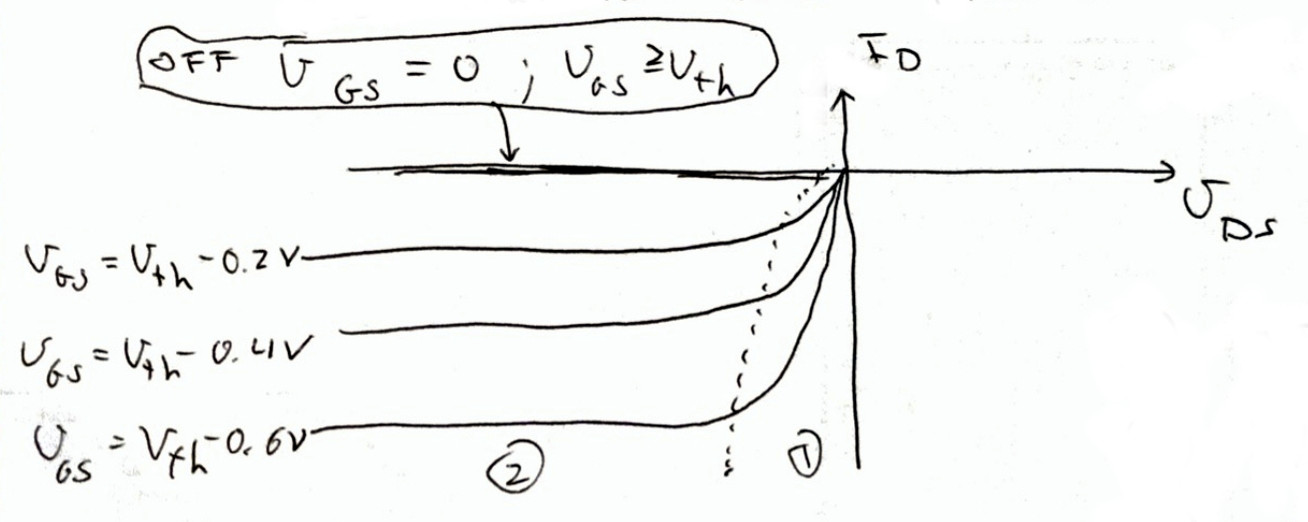
\includegraphics[width=\linewidth]{figures/PMOS-IV}
  \caption{I-V characteristic of a \textsc{PMOS} transistor at different values of \(v_\text{GS}\).}
  \label{figure:lec2-PMOS-IV}
\end{figure}
Another kind of \textsc{mosfet} is the \textsc{pmos}.
They have a similar construction as \textsc{nmos} transistors, but their
behavior is opposite, and for the ``on'' condition of \(V_\text{GS} < V_\text{t,p}\), \(V_\text{t,p} < 0\).
\autoref{figure:lec2-PMOS} and \autoref{figure:lec2-PMOS-IV}
are the counterparts of \autoref{figure:lec2-NMOS} and
\autoref{figure:lec2-NMOS-IV}, respectively.

For most of this class, we'll use more idealized models
of these transistors in digital logic settings.
In the voltage-controlled switch perspective,
\textsc{nmos} transistors open at lower voltages and close at higher voltages,
and \textsc{pmos} transistors close at lower voltages and open at high ones.

\section{An \textsc{nmos} inverter}
One building block we need to understand digital logic is the \emph{inverter},
which is a circuit that outputs a high voltage when its input is a low
voltage, and vice versa.
The high voltage represents a digital value of 1 (true), and the low voltage represents a digital value of 0 (false).

It's possible to build an inverter using an \textsc{nmos} transistor,
as shown in \autoref{figure:lec2-NMOS-inverter}.
The high voltage is called \(V_\text{DD}\), which stands for
the voltage supplied by the high power rail,
and in this example has a value of 1 volt.%
\footnote{For obscure historical reasons.}
In this example, our reference voltage will be ground---0 volts.

\begin{figure}
  \centering
  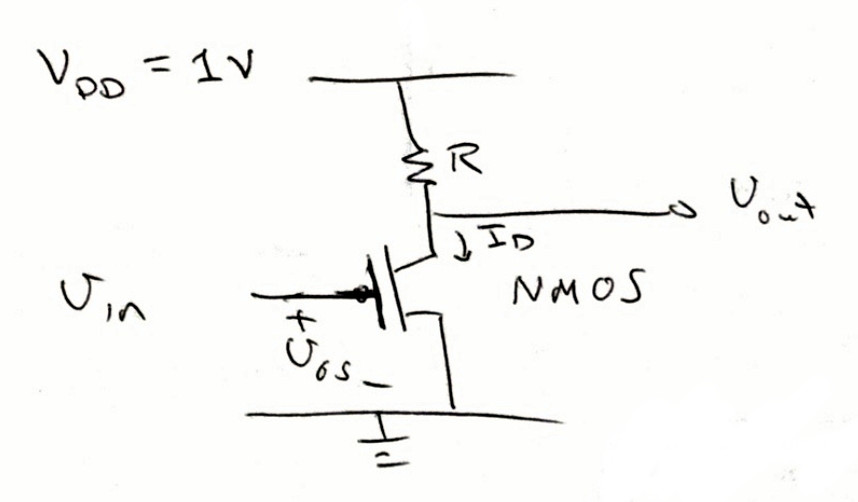
\includegraphics[width=0.75\linewidth]{figures/NMOS-inverter}
  \caption{A inverter built using an \textsc{nmos} transistor.}
  \label{figure:lec2-NMOS-inverter}
\end{figure}

\subsection{Analysis}
\begin{itemize}
\item
(Case \(v_\text{in} = 0\))
The transistor, as a switch, is off.
As a result, the terminal \(v_\text{out}\)
is connected directly to \(V_\text{DD}\) by a resistor.
Because no current flows into the voltage terminal,
by Ohm's law there can be no voltage drop across the resistor.
Therefore \(v_\text{out} = V_\text{DD}\).

\item
(Case \(v_\text{in} = V_\text{DD}\))
The transistor, as a switch, is on. The terminal \(v_\text{out}\) has a short to ground, so \(v_\text{out} = 0\).
\end{itemize}

\autoref{figure:lec2-inverter-truth-table} shows
the truth table of this circuit and verifies that this circuit is indeed
an inverter.

\begin{figure}
  \centering
  \begin{tabular}{ll}
    \(v_\text{in}\) & \(v_\text{out}\) \\\hline
    0 & \(V_\text{DD}\)\\
    \(V_\text{DD}\) & 0
  \end{tabular}
  \caption{Truth table of the \textsc{nmos} inverter.}
  \label{figure:lec2-inverter-truth-table}
\end{figure}

\subsection{Power consumption}
When \(v_\text{in} = 0\), the circuit consumes no power, as we have established that there is no current through the resistor between \(V_\text{DD}\) and \(v_\text{out}\).
When \(v_\text{in} = V_\text{DD}\), there is a path from \(V_\text{DD}\) through the resistor, then the transistor, to ground.
The circuit consumes power \(VI = {V_\text{DD}^2}/{R}\).
While this might not necessarily be a lot, in computing applications with countless transistors, it adds up, and moving heat away from a dense circuit poses engineering challenges.
Dense digital circuits were made possible by the discovery of the CMOS inverter architecture, which avoids a path from \(V_\text{DD}\) to ground.

\section{A \textsc{cmos} inverter}
\begin{figure}
  \centering
  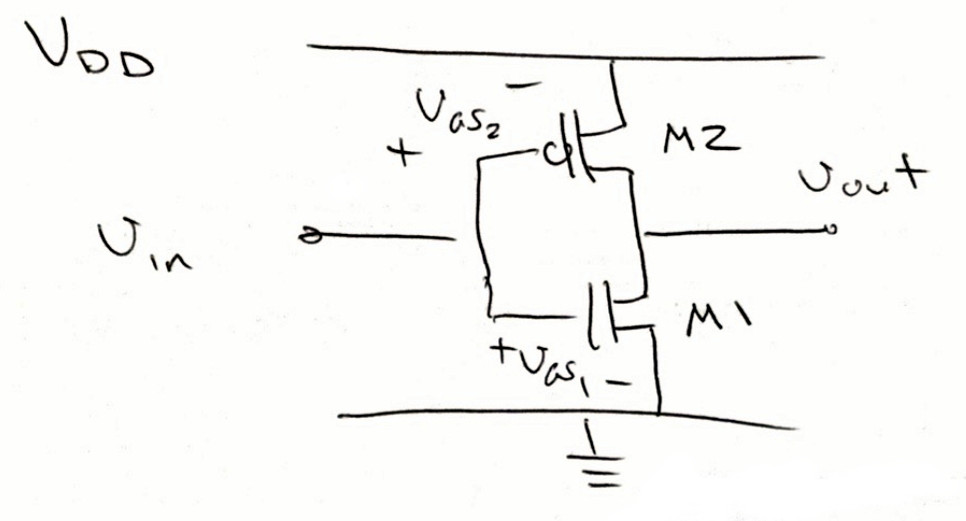
\includegraphics[width=0.75\linewidth]{figures/CMOS-inverter}
  \caption{A inverter built using the \textsc{cmos} design..}
  \label{figure:lec2-CMOS-inverter}
\end{figure}

\autoref{figure:lec2-CMOS-inverter} shows an inverter circuit that exemplifies the \textsc{\em cmos} design strategy of using \textsc{pmos} and \textsc{nmos} transistors together.

\begin{figure}
  \centering
  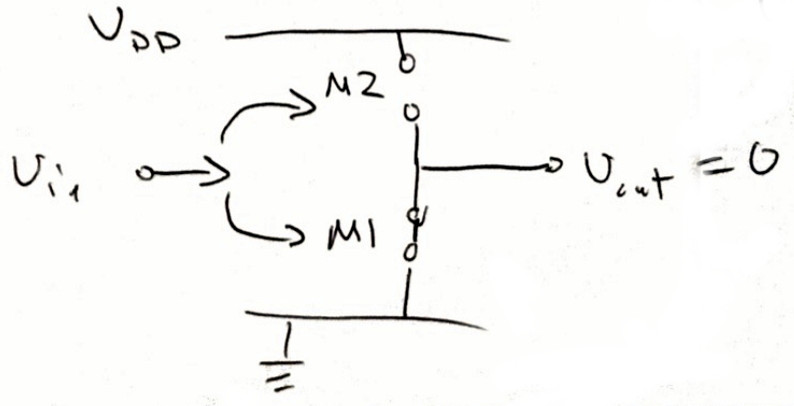
\includegraphics[width=0.75\linewidth]{figures/CMOS-case}
  \caption{Equivalent circuit of \autoref{figure:lec2-CMOS-inverter}
  when \(v_\text{in} = V_\text{DD}\).}
  \label{figure:lec2-CMOS-case}
\end{figure}

\subsection{Analysis}
\begin{itemize}
  \item
  (Case \(v_\text{in} = V_\text{DD}\))
  \begin{itemize}
    \item
    The \textsc{pmos} having as its source \(V_\text{DD}\) and \(v_\text{out}\) as its drain
    \(V_\text{GS,1} = 0\), which is higher than \(V_\text{t,p}\).
    Therefore there is no path from \(V_\text{DD}\) to \(v_\text{out}\).
    \item
    The \textsc{nmos} having \(v_\text{out}\) as its drain and ground as its source has \(V_\text{GS,2}= V_\text{DD}\),
    which is higher than \(V_\text{t,n}\).
    Therefore, due to the terminal's short to ground, \(v_\text{out} = 0\).
  \end{itemize}
  The equivalent circuit once the switch model has been applied is shown in  \autoref{figure:lec2-CMOS-case}.

  \item
  (Case \(v_\text{in} = 0\))
  \begin{itemize}
      \item
      The \textsc{pmos}, having \(V_\text{GS,1} = -V_\text{DD} < V_\text{t,p}\), turns on.
      \item
      The \textsc{nmos}, having \(V_\text{GS,2} = 0 < V_\text{t,n}\), turns off.
  \end{itemize}
  Therefore \(V_\text{out} = V_\text{DD}\).
\end{itemize}

\subsection{Power consumption}
All currents are zero in this model, so no power is consumed.

\section{A \textsc{cmos} inverter chain with capacitance}
\begin{figure}
  \centering
  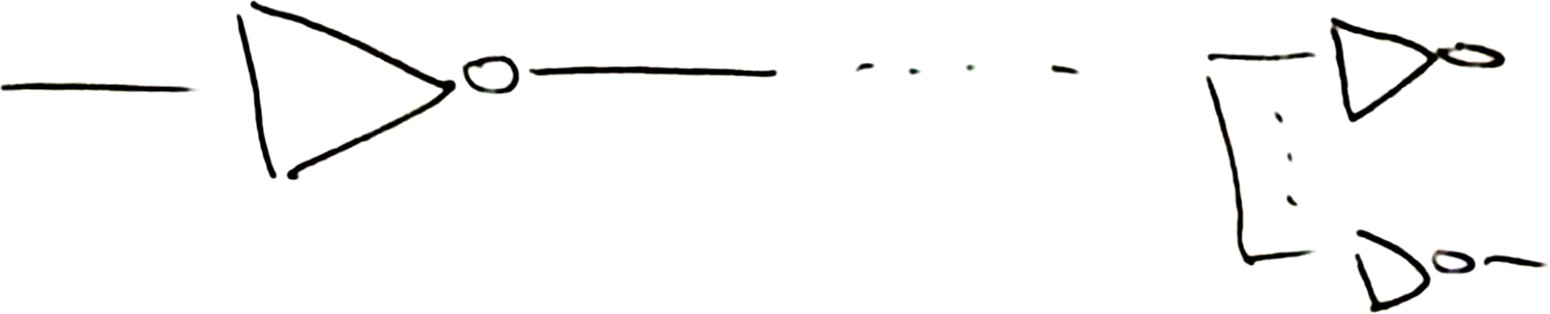
\includegraphics[width=0.75\linewidth]{figures/inverter-chain}
  \caption{A chain of inverters, which is kind of similar to a computer.}
  \label{figure:lec2-inverter-chain}
\end{figure}
Contrary to our last conclusion, inverters in real electronics certainly do consume some power.
We'll pretend digital circuits are chains of inverters (\autoref{figure:lec2-inverter-chain})---although this model won't teach you how to build a computer, it is close enough to real \textsc{cmos} networks to illustrate when and where power is expended.

We will concentrate our analysis on just one stage of the \textsc{cmos} inverter chain.
A single inverter is shown in \autoref{figure:lec2-CMOS-cap},
with a capacitor between \(v_\text{out}\) and ground to model the
next stage's load.
\begin{figure}
  \centering
  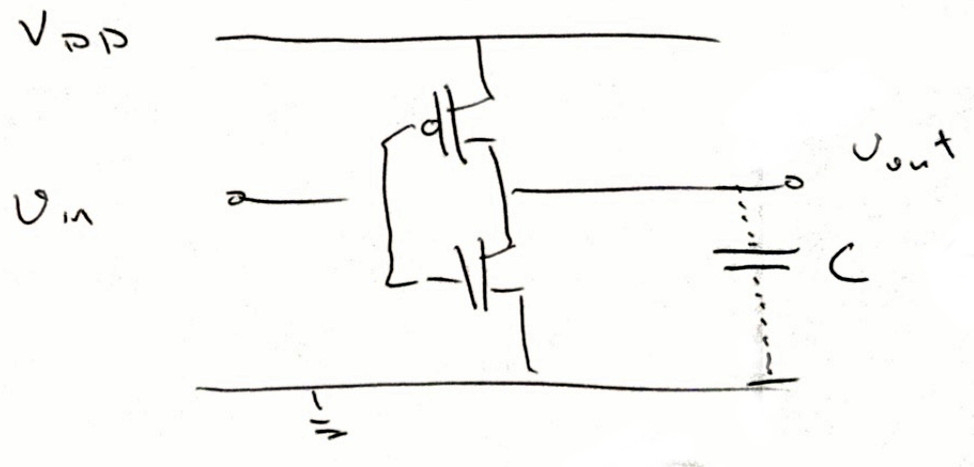
\includegraphics[width=0.75\linewidth]{figures/CMOS-inverter-with-out-cap}
  \caption{An inverter taken from a chain with a capacitor modeling the next stage.}
  \label{figure:lec2-CMOS-cap}
\end{figure}
\autoref{figure:lec2-CMOS-cap-1} shows the equivalent circuit when the output of this inverter settles at \(V_\text{DD}\).
\begin{figure}
  \centering
  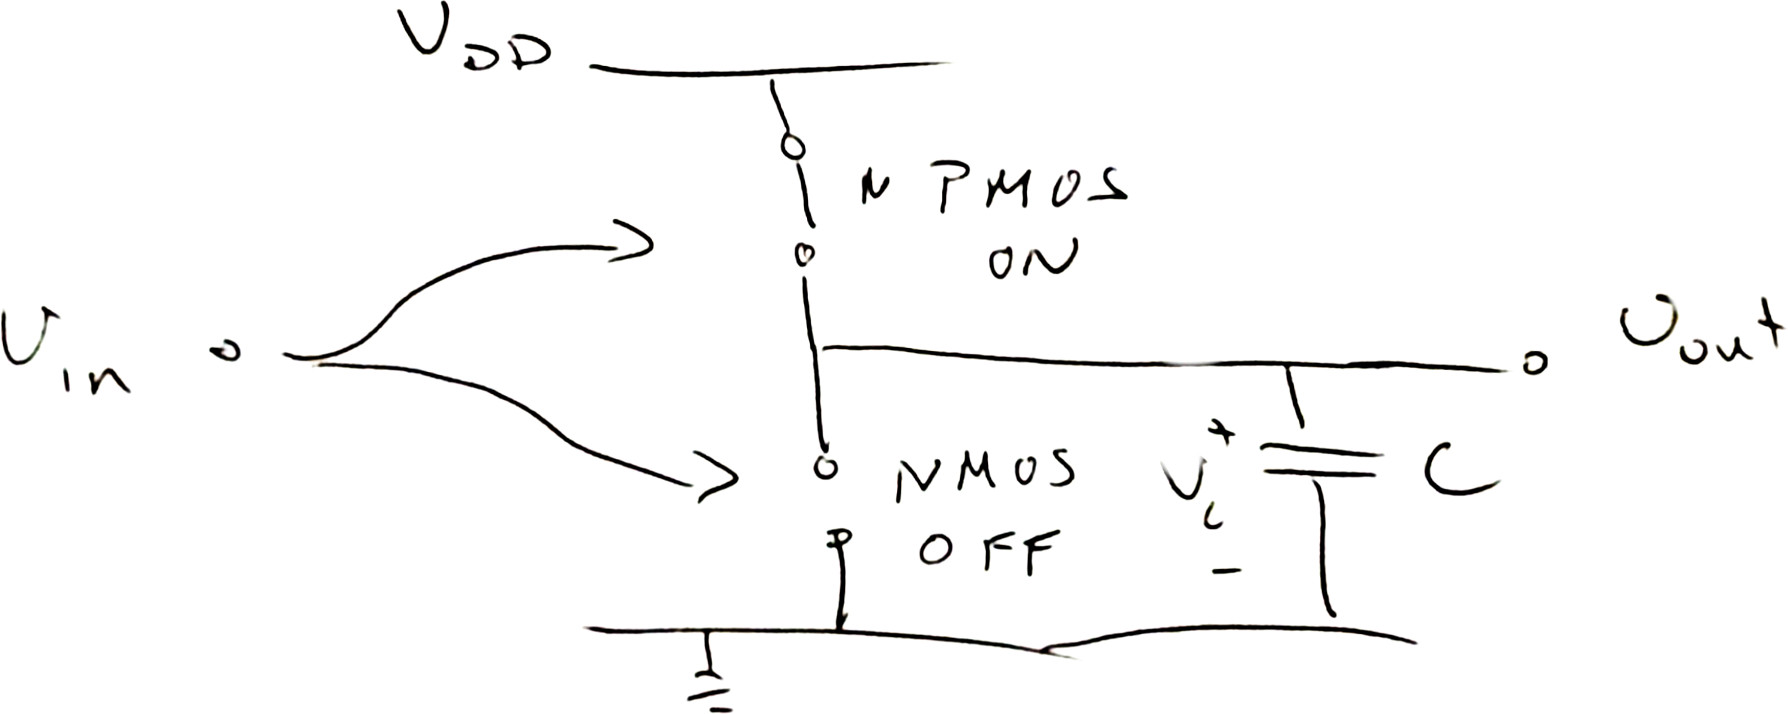
\includegraphics[width=0.75\linewidth]{figures/CMOS-cap-1}
  \caption{An inverter outputting \(V_\text{DD}\) with load capacitor.}
  \label{figure:lec2-CMOS-cap-1}
\end{figure}

\subsection{Potential energy in a capacitor}
\begin{figure}
  \centering
  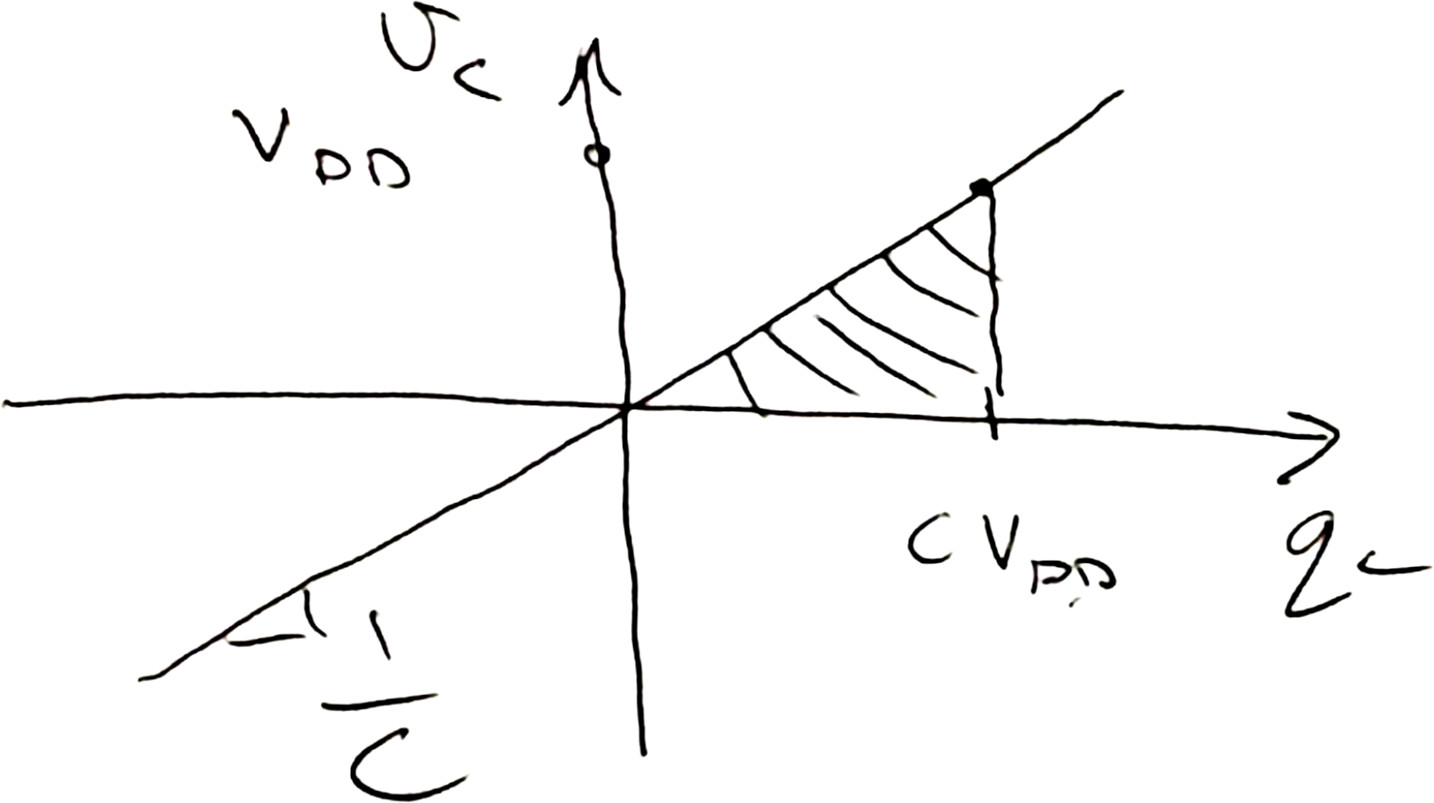
\includegraphics[width=0.75\linewidth]{figures/cap-energy-integral}
  \caption{Energy stored in a capacitor can be computed by an integral under the \(V = Q/C\) curve.}
  \label{figure:lec2-cap-energy-integral}
\end{figure}
The energy stored in the capacitor when it has voltage \(V_\text{DD}\) is given by the formula
\begin{align}
  E_\text{cap}
  &= \frac{1}{2} CV_\text{DD}^2,
\end{align}
which can be derived by using the facts that 1) that voltage is energy per unit charge and 2) a capacitor obeys \(Q = CV\), and integrating through the total charge stored in the capacitor: \(\int_0^{CV_\text{DD}} v_C \dif q\) (\autoref{figure:lec2-cap-energy-integral}).

\begin{figure}
  \centering
  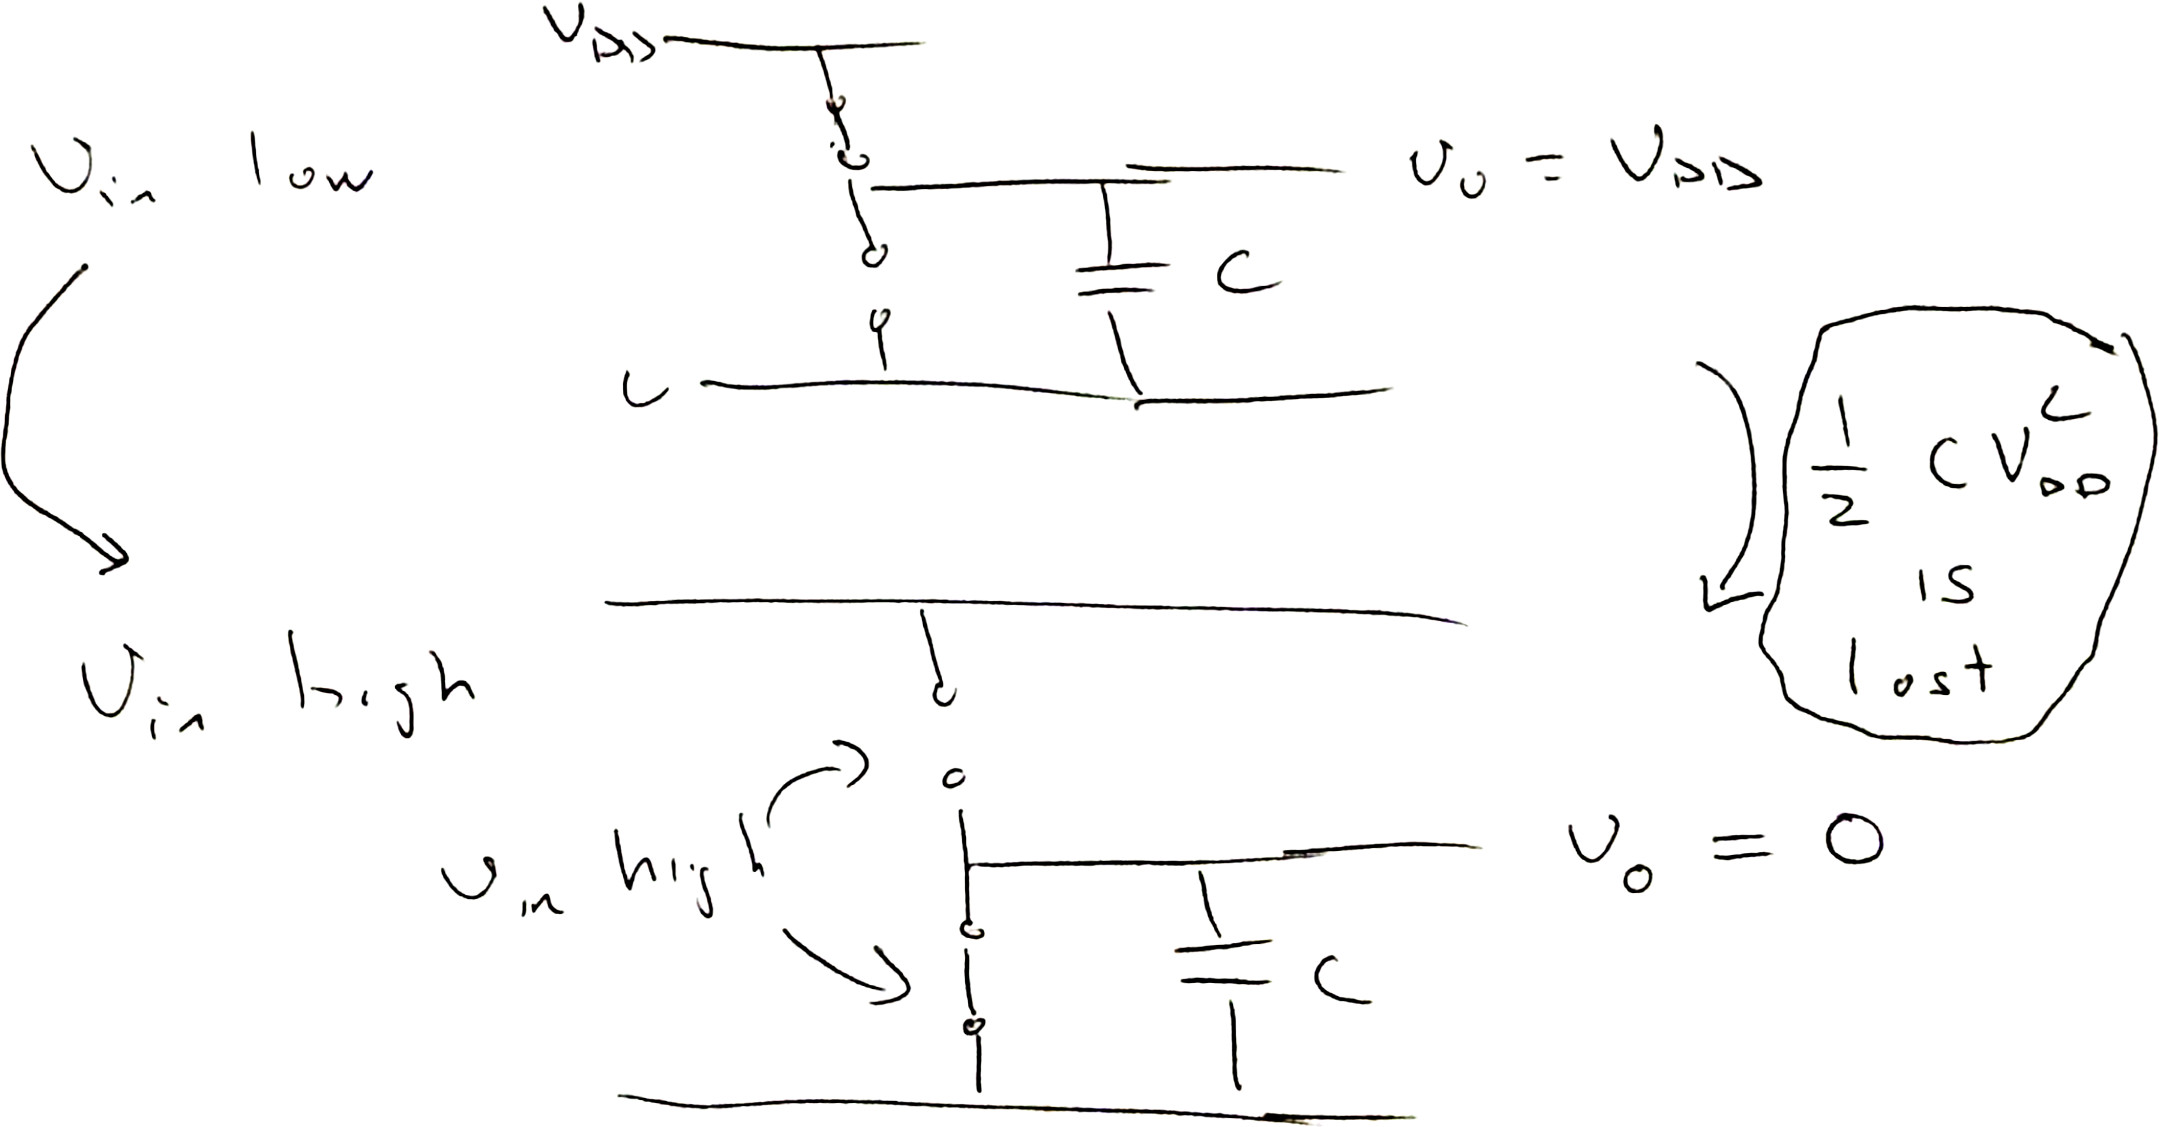
\includegraphics[width=1\linewidth]{figures/cap-discharge-energy}
  \caption{\textsc{cmos} load capacitor forced from voltage \(V_\text{DD}\) to \(0\).}
  \label{figure:lec2-cap-discharge-energy}
\end{figure}
When the inverter's input changes from low to high, the output must change from \(V_\text{DD}\) to \(0\) (\autoref{figure:lec2-cap-discharge-energy}).
That means that the load capacitor must discharge fully, burning \(\frac{1}{2}CV_\text{DD}^2\) of potential energy as heat.

\subsection{Total energy supplied}
Even though the capacitor only stores and discharges
\(\frac{1}{2}CV_\text{DD}^2\),
an up-down cycle costs \(CV_\text{DD}^2\).
This is because the voltage source must offer \(Q = CV_\text{DD}\) of charge
at \(V_\text{DD}\) energy per unit charge.
Where does this go? Let's follow the energy as the output changes from 0 to 1 and back to 0.
\begin{enumerate}
  \item (\(q_C = 0\), \(v_C = 0\))
  \item Voltage source loads \(CV_\text{DD}\) of charge at \(V_\text{DD}\) energy per unit charge, at a total expense of \(CV_\text{DD}^2\).
  Half of its energy output is burned by ``parasitic'' resistance en route to the capacitor, and the other half is stored in the capacitor.
  \item (\(q_C = CV_\text{DD}\), \(v_C = V_\text{DD}\))
  \item Transistors toggle, and the capacitor drains, generating \(\frac{1}{2} CV_\text{DD}^2\) of heat on the pull-down circuit.
  \item (\(q_C = 0\), \(v_C = 0\))
\end{enumerate}

\subsection{Where does the energy in a device go?}
With reference to our chain-of-inverters model,
power consumption in digital devices is mainly explained by three phenomena:
\begin{itemize}
  \item If the inverter flips every cycle at a clock speed of \(f_s\),
  the circuit will burn \(f_sCV_\text{DD}^2\) charging its capacitors.
  \item Leakage: a transistor that's ``off'' isn't 100\% off, and a small amount of current flows and burns some energy.
  \item Short-circuit current (smaller): when the input is flipping between 0 and 1, there's a very short instant during which both transistors may be \emph{on}, and some current flows through the momentary \(V_\text{DD}\)-ground short.
\end{itemize}

\chapter{Transient Analysis}
% TODO (possibly)
% Some material introducing the dielectrics inside a MOSFET transistor
% in order to motivate transients has been left out.
(For this lecture, a \textsc{mosfet} transistor is considered to transition between ``on'' and ``off'' at \(v_\text{GS} = \frac{1}{2} V_\text{DD}\).)

\begin{figure}
  \centering
  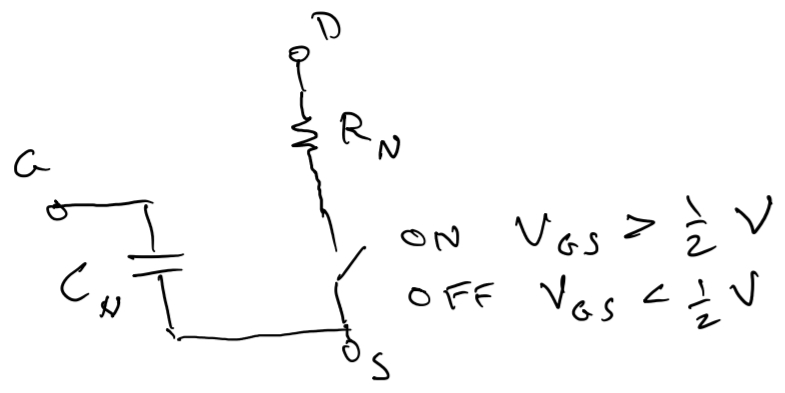
\includegraphics[width=0.75\linewidth]{figures/3/nmos-cap}
  \caption{Model of \textsc{nmos} transistor with G-S capacitance.}
  \label{figure:lec3-nmos-cap}
\end{figure}
\begin{figure}
  \centering
  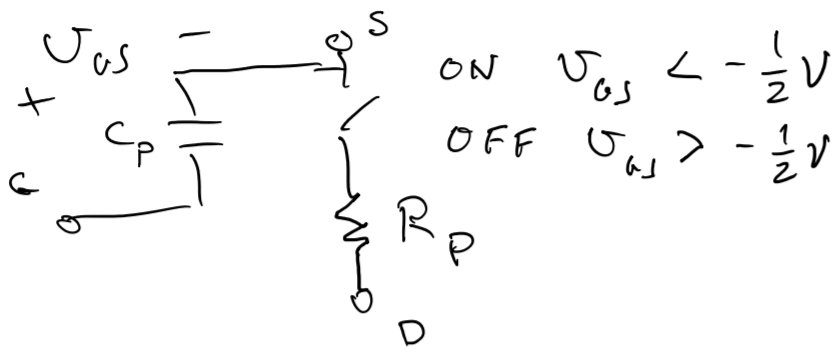
\includegraphics[width=0.75\linewidth]{figures/3/pmos-cap}
  \caption{Model of \textsc{pmos} transistor with G-S capacitance.}
  \label{figure:lec3-pmos-cap}
\end{figure}
We'll enrich our analog model of \textsc{mosfet}s as voltage-controlled switches by acknowledging capacitance between the \textsc{mosfet}'s gate and source.
\autoref{figure:lec3-nmos-cap} and \autoref{figure:lec3-pmos-cap}
depict \textsc{nmos} and \textsc{pmos} transistors in this model.

\begin{figure}
  \centering
  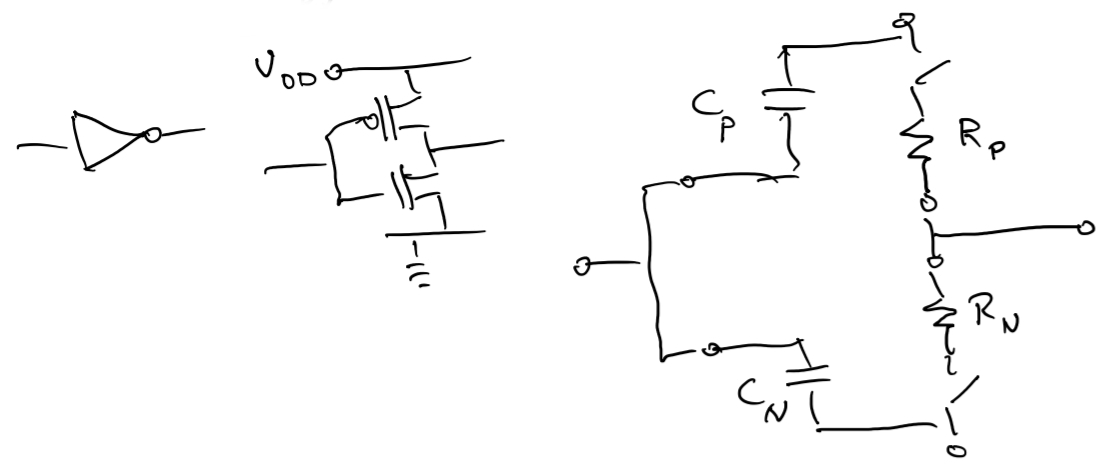
\includegraphics[width=0.75\linewidth]{figures/3/3inverters}
  \caption{A \textsc{cmos} inverter at three levels of abstraction.}
  \label{figure:lec3-3inverters}
\end{figure}
\autoref{figure:lec3-3inverters} summarizes the three levels of abstraction with which we are able to reason about \textsc{cmos} inverters.
On the very left is a digital symbol for an inverter that hides how the inverter works.
In the center is the construction of an inverter using complementary \textsc{mosfet}s.
On the right is a fairly faithful analog representation of an inverter that will allow us to interrogate the assumptions that, thus far, have enabled us to treat the analog circuit as a digital one.

\section{RC transient in an inverter chain}
Let's return to the case study of a chain of inverters, this time focusing on just two consecutive inverters.
\begin{figure}
  \centering
  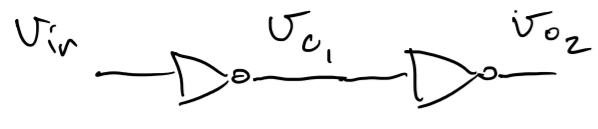
\includegraphics[width=0.75\linewidth]{figures/3/inverter-chain}
  \caption{Two consecutive \textsc{cmos} inverters, part of a longer chain.}
  \label{figure:lec3-inverter-chain}
\end{figure}
In \autoref{figure:lec3-inverter-chain} three wires are labeled as follows:
\begin{itemize}
  \item \(v_\text{in}\) is the input to the first inverter,
  \item \(v_{\text{o}_1}\) is the output of the first inverter (and the input to the second), and
  \item \(v_{\text{o}_2}\) is the output of the second.
\end{itemize}
The digital logic interpretation is that \(v_{\text{o}_2}\) is the double negation of \(v_\text{in}\), that is, \(v_{\text{o}_2} = v_\text{in}\).

\begin{figure}
  \centering
  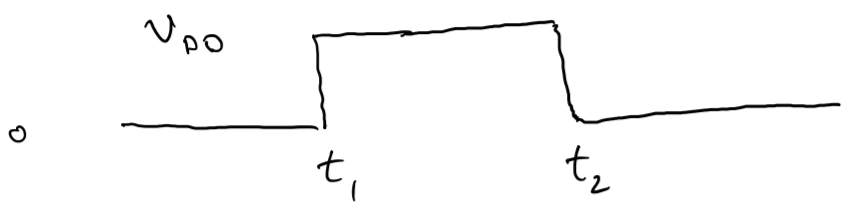
\includegraphics[width=0.75\linewidth]{figures/3/input-signal}
  \caption{Input signal to the first inverter of \autoref{figure:lec3-inverter-chain}}
  \label{figure:lec3-input-signal}
\end{figure}
We will study what happens when \(v_\text{in}\) is driven by the input depicted in \autoref{figure:lec3-input-signal}. It will begin having remained at 0 for a long time, change to \(v_\text{DD}\) at time \(t_1\), then return to \(0\) at time \(t_2 > t_1\).
\begin{figure}
  \centering
  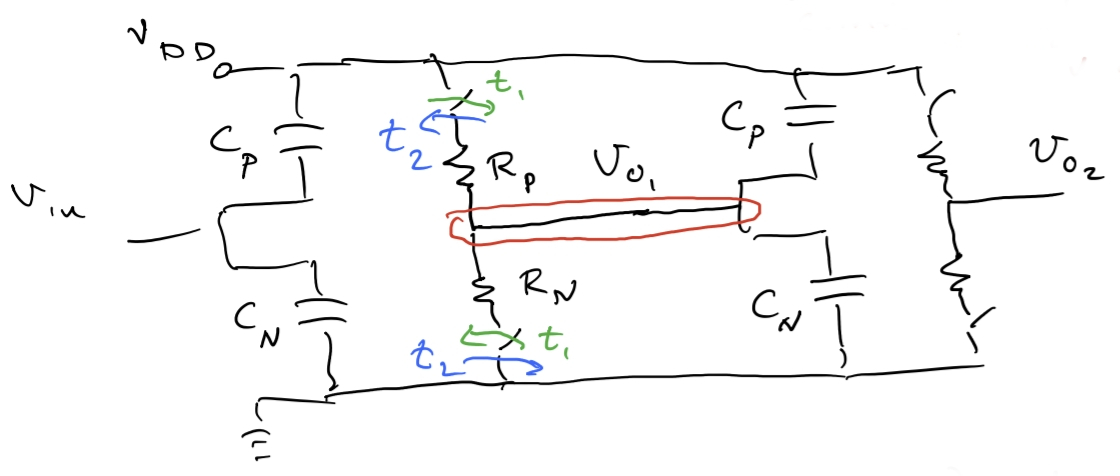
\includegraphics[width=1\linewidth]{figures/3/chain-RC}
  \caption{Analog redrawing of \autoref{figure:lec3-inverter-chain}, showing switch actions of the first inverter, as well as a distinguished node.}
  \label{figure:lec3-chain-RC}
\end{figure}
\autoref{figure:lec3-chain-RC} shows the actions of the switches of the first inverter's transistors at times \(t_1\) and \(t_2\).
For the rest of this section, we'll just concentrate on what happens to \(v_{\text{o}_1}\).

\subsection{Before \(t_1\)}
As \(v_\text{in} = 0\) well before \(t_1\), we can assume that the circuit has settled, and the output of the first inverter is \(v_\text{DD}\).

\subsection{After \(t_1\), before \(t_2\)}
At \(t_1\), the pull-up switch opens, and the pull-down switch closes.
KCL applied to the distinguished (red) middle node of \autoref{figure:lec3-chain-RC} requires the outgoing currents to sum to zero.
Using Ohm's Law once and the capacitor current-voltage relationship twice, we have the following equation:
\begin{align}
  \frac{v_{\text{o}_1}}{R_N}
  + C_N \dod{}{t} v_{\text{o}_1}
  + C_P \dod{}{t} \del{v_{\text{o}_1} - v_\text{DD}}
  &= 0 \\
  \dod{}{t} v_{\text{o}_1}
  + \frac{1}{R_N \del{C_N + C_P}} v_{\text{o}_1}
  &= 0\\
  \intertext{
  This is a differential equation that we will analyze with initial condition \(v_{\text{o}_1}(t_1) = V_\text{DD}\).
  For equations of this sort we will identify a characteristic quantity \(\tau\) as follows:
  }
  \tau &= R_N \del{C_N + C_P}
  \intertext{
  The International System of Units means that \(\tau\) is measured in Ohm-Farads, or seconds.
  For this reason, \(\tau\) is called the \emph{time constant} of the system.
  A time constant on the order of tens of picoseconds is considered state-of-the-art for modern devices, arising from resistances on the order of kiloOhms and capacitances on the order of femtofarads. Rewriting using \(\tau\),
  }
  \dod{}{t} v_{\text{o}_1}
  &= - \frac{1}{\tau} v_{\text{o}_1}\\
  \intertext{
  We will refer to the constant of proportionality between \(\od{}{t} v_{\text{o}_1}\) and \(v_{\text{o}_1}\) as \(\lambda\).
  }
  \dod{}{t} v_{\text{o}_1}
  &= \lambda v_{\text{o}_1}
  \intertext{
  There are many heuristic techniques to propose a solution to this differential equation. One of them is called Separation of Variables, which involves equations such as
  \(\int \frac{\dif v_{\text{o}_1}}{v_{\text{o}_1}} = \int \lambda \dif t\).
  The resulting solution form, where \(A\) is a constant that remains to be determined, is all that you will need to know about this variety of differential equation:
  }
  v_{\text{o}_1}(t)
  &= A e^{\lambda t}
  \intertext{
  (As an aside, you can verify that
  \(v_{\text{o}_1}(t) = A e^{\lambda t}\)
  is a solution---
  differentiating both sides with respect to \(t\) results in
  \(\od{}{t} v_{\text{o}_1}(t) = A \lambda e^{\lambda t} = \lambda (A e^{\lambda t})\).)
  Our next goal is to determine \(A\).
  We can do so by choosing \(A\) to meet the initial condition
  \(v_{\text{o}_1}(t_1) = V_\text{DD}\).
  Substituting \(v_{\text{o}_1}(t) = A e^{\lambda t}\),
  }
  A e^{\lambda t_1} &= V_\text{DD} \\
  A &= V_\text{DD} e^{-\lambda t_1} \\
  v_{\text{o}_1}
  &= \del{V_\text{DD} e^{-\lambda t_1}} e^{\lambda t} \\
  &= V_\text{DD} e^{-\del{\frac{t - t_1}{\tau}}}
\end{align}

\begin{figure}
  \centering
  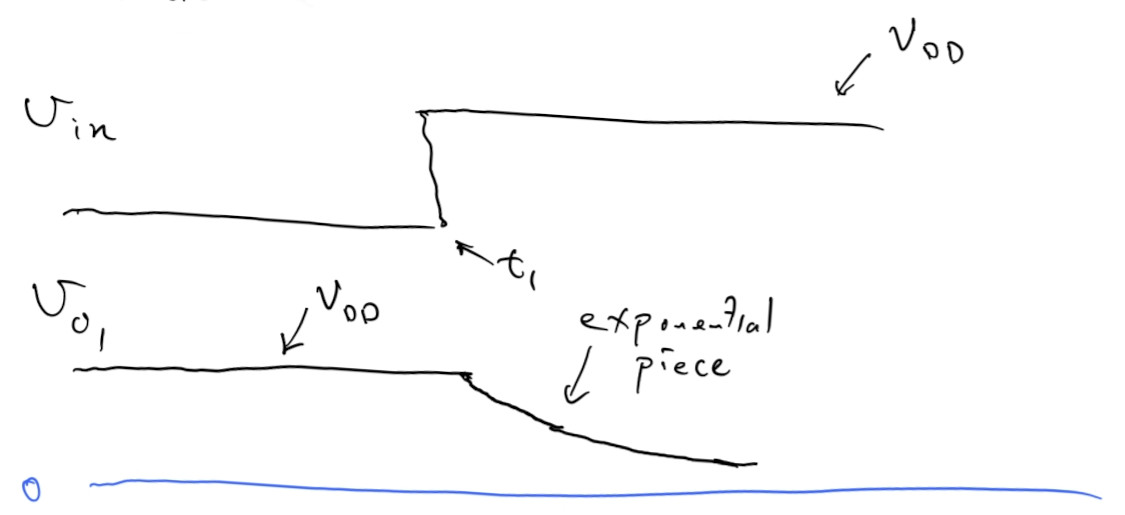
\includegraphics[width=\linewidth]{figures/3/exponential-sketch}
  \caption{Sketch of transient from \(t_1\) to \(t_2\) in \autoref{figure:lec3-chain-RC}.}
  \label{figure:lec3-transient}
\end{figure}
\autoref{figure:lec3-transient} is a sketch of \(v_\text{in}\) and \(v_{\text{o}_1}\) after \(t_1\) and before \(t_2\).
Notice that \(v_{\text{o}_1}\) doesn't immediately jump to \(0\) like the digital model assumes.
Rather, \(v_{\text{o}_1}\) decays exponentially toward 0 at a rate predicted by \(\tau\).
Discharging a capacitor takes time, and digital devices' clock speed is limited by how quickly binary values settle in between logic gates.


\subsection{After \(t_2\)}
We will try to write a differential equation describing the evolution of \(v_{\text{o}_1}\) at time \(t_2\) and beyond.
\autoref{figure:lec3-chain-RC} shows that at time \(t_2\), the pull-up switch closes, and the pull-down switch opens.
KCL applied to the same central node yields the following differential equation:
\begin{align}
  \frac{v_{\text{o}_1} - V_\text{DD}}{R_P}
  + \del{C_P + C_N} \dod{}{t} v_{\text{o}_1}
  &= 0\\
  \dod{}{t} v_{\text{o}_1}
  + \frac{1}{R_P\del{C_P + C_N}} v_{\text{o}_1}
  &= \frac{v_\text{DD}}{R_P \del{C_P + C_N}}
  \intertext{
  The previous solution for \(v_{\text{o}_1}\), which is valid up until time \(t_2\), may be evaluated at \(t_2\) for a boundary condition valid past \(t_2\):
  }
  v_{\text{o}_1}(t_2)
  &= V_\text{DD} e^{-\del{\frac{t_2 - t_1}{\tau}}}\\
  \intertext{
  A solution for \(v_{\text{o}_1}\) from \(t_2\) onwards is:
  }
  v_{\text{o}_1}
  &= V_\text{DD} + \del{v_{\text{o}_1}(t_2) - V_\text{DD}}
  e^{-\del{\frac{t - t_2}{\tau_P}}},
\end{align}
where \(\tau_P = R_P\del{C_P + C_N}\).
%% TODO: explain this?

\section{Uniqueness}
We solved a differential equation. Differential equations are universal and ubiquitous in science and engineering.

A theorem states that a large class of differential equations with boundary conditions have unique solutions. These differential equations are of the form
\begin{align}
  \dod{}{t} x
  &= f(x, t), \quad x(0) = x_0,
\end{align}
where
\begin{enumerate}
  \item
  for all values of \(t\), \(f(x, t)\) is differentiable with respect to \(x\) and
  \(\left| \pd{f}{x} (x,t) \right| < M\) for some nonnegative real number \(M\); and
  \item for all values of \(x\), \(f(x,t)\) has a finite number of discontinuities in \(t\) in any unit interval \([t_0, t_0 + 1]\).
\end{enumerate}
If these conditions hold, then our differential equation has a unique solution.

Note that these conditions are in fact quite loose, and are more than enough to certify that unique solutions exist to differential equations of the form \(\od{}{t} x = f(x) = \lambda x\).
It is important that we have proofs of existence and uniqueness because methods such as Separation of Variables are not inherently rigorous.
Only once we have verifed that a proposed solution satisfies the differential equation and boundary condition may we claim that it is a solution.
Because these problems have unique solutions, we may be certain that the model we are using is physically deterministic---it tells precisely what must happen, not just what \emph{may} happen.

\chapter{Differential equations with inputs}
\section{RC with exponential input}
\begin{figure}
  \centering
  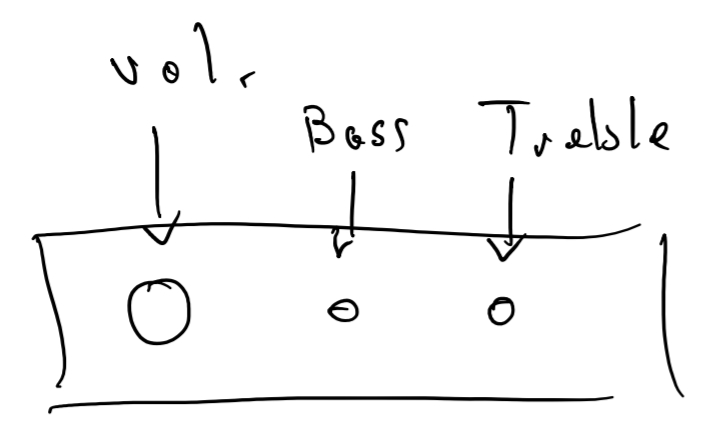
\includegraphics[width=0.5\linewidth]{figures/4/amp}
  \caption{An amp with three knobs to adjust playback.}
  \label{figure:lec4-amp}
\end{figure}
\begin{figure}
  \centering
  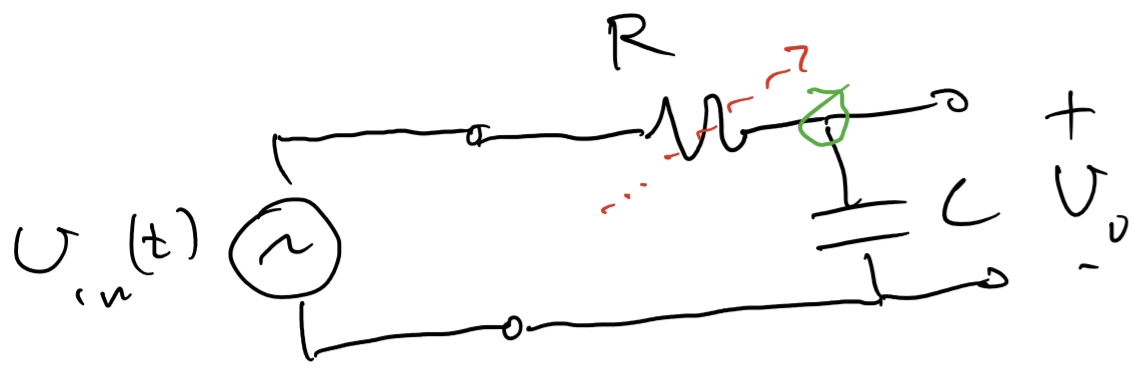
\includegraphics[width=1\linewidth]{figures/4/RC}
  \caption{RC circuit as a filter.}
  \label{figure:lec4-RC}
\end{figure}

In this section we will derive, in a more hands-on way, the behavior of an RC circuit forced by an exponential input.
If you have ever used an amp%
% \footnote{Specifically, a less-cool solid-state one.}
with knobs for treble and bass (\autoref{figure:lec4-amp}), then you have interacted with two circuits
similar to the one shown in \autoref{figure:lec4-RC}.
The resistor with a arrow is a variable resistor, or potentiometer,%
\footnote{Electric guitars use this circuit component, which guitarists call ``pots,'' to blend the pickups' signals.}
that might be controlled by one of the amp's knobs.

In \autoref{figure:lec4-RC},
\begin{itemize}
  \item \(v_\text{in}\) represents the amp's analog input,
  \item \(v_o\) is used to drive the speakers after subsequent amplification, and
  \item \(R\) represents the setting on one of the potentiometers.
\end{itemize}
By studying the distinguished (green) node, we can write the following differential equation:
\begin{align}
  \label{eqn:lec4-RC}
  \dod{}{t} v_o(t)
  &= -\frac{1}{RC} v_o(t) + \frac{1}{RC} v_\text{in}(t).
  \intertext{We'll constrain \(v_\text{in}\) to have the following form:}
  v_\text{in}(t)
  &= V_\text{in} e^{st}.
  \intertext{While it seems that this form is arbitrary, it will prove  insightful, because \(e^{st}\) is an \emph{eigenfunction} for input-output behavior of this circuit, i.e.\ we expect}
  v_o(t) &= V_o e^{st}.
  \intertext{We can determine \(V_o\) by substituting our parameterization of \(v_o\) into \autoref{eqn:lec4-RC}, whose LHS\ldots}
  \dod{}{t} v_o(t)
  &= \dod{}{t} V_o e^{st} \\
  &= sV_o e^{st}
  \intertext{\ldots is equated with the RHS:}
  sV_o e^{st}
  &= -\frac{1}{RC} V_o e^{st} + \frac{1}{RC} V_\text{in} e^{st}.
  \intertext{Now we can isolate \(V_o\).}
  sV_0 + \frac{1}{RC} V_o
  &= \frac{1}{RC} V_\text{in} \\
  V_o
  &= \del{\frac{1}{RC}} \del{\frac{1}{s + \frac{1}{RC}}} V_\text{in}
  \intertext{Substituting \(\lambda = -\frac{1}{RC}\),}
  V_o
  &= \frac{1}{1 - \frac{s}{\lambda}} V_\text{in}
  \intertext{All together, our solution for \(v_o(t)\) is the following:}
  v_o(t) = V_o e^{st}
  &= \frac{1}{1 - \frac{s}{\lambda}} V_\text{in} e^{st}.
  \intertext{Suppose that we have an initial condition for \(v_o\) at time 0.}
  \eval{ v_o }_{t = 0}
  &= v_1
  \intertext{Then our solution, taking this fact into account, will be}
  v_o(t) &= A e^{-\frac{t}{RC}} +
  \frac{1}{RC}
    \del{\frac{V_\text{in} e^{st}}{s + \frac{1}{RC}}},
  \intertext{where \(A\) remains to be determined, viz.\ by evaluating both sides at \(t = 0\):}
  v_1 &= A + \frac{1}{RC} \del{\frac{V_\text{in}}{s + \frac{1}{RC}}}\\
  A &= v_1 - \frac{1}{RC} \del{\frac{V_\text{in}}{s + \frac{1}{RC}}}.
  \intertext{This concludes our example. A solution to a linear differential equation will, generally, have the following structure:}
  v(t)
  &= v_\text{homogeneous}(t) + v_\text{particular}(t),
  \intertext{where \(v_\text{homogeneous}(t)\) corresponds to the initial condition, and \(v_\text{particular}(t)\) to the input term.}
\end{align}

\section{General scalar differential equation}
We will verify that the following general differential equation:
\begin{align}
  \label{eqn:lec4-general-diffeq}
  \dod{}{t} x(t)
  &= \lambda x(t) + u(t); \quad x(t_0) = x_0
  \intertext{has the following solution, which is a sum of a homogeneous and a particular term:}
  x(t)
  &= e^{\lambda(t - t_0)} x_0
  + \int_{t_0}^t e^{\lambda (t - \tau)} u(\tau) \dif \tau.
  \intertext{We can check the initial condition \(x(t_0) = x_0\): the former term evaluates to \(x_0\) and the latter to \(0\).
  Next, we can verify that
  \(\od{}{t} x(t)
  = \lambda x(t) + u(t)\) holds by differentiating.}
  \dod{}{t} x(t)
  &= \bigg\{ \lambda e^{\lambda (t - t_0)}
             x_0
           \bigg\} +
  u(t) +
  \bigg\{
    \int_{t_0}^{t} \lambda e^{\lambda (t - \tau) } u(\tau) \dif \tau
  \bigg\}
\end{align}
% (The latter two terms result from Leibniz's rule for differenting definite integrals.)
The two terms in curly braces sum to \(\lambda x(t)\), so \autoref{eqn:lec4-general-diffeq} is satisfied.

\chapter{Vector differential equations and second-order circuits}

\section{Guess-and-check for RC filter with cosine input}
Last lecture we derived the folowing equation modeling the input-output properties of an amp: (where \(R\) is set by a potentiometer)
\begin{align}
  \dod{}{t} v_\text{out}(t)
  &= -\frac{1}{RC} v_\text{out}(t) + \frac{1}{RC} v_\text{in}(t);
  \quad \left.v_\text{out} \right|_{t_0} = V
  \intertext{
  In this section we will try to determine the result in \(v_\text{out}\) when \(v_\text{in}\) has the following sinusoidal form:
  }
  v_\text{in}(t)
  &= V_\text{in} \cos\del{\omega t}
  \intertext{This defines a sinusoid with amplitude \(V_\text{in}\) and a frequency of \(\omega\), which is angular frequency, in \(\unit{rad}/\unit{s}\).
  Angular frequency is related to cycles/second by \(\omega = 2\pi f\), where \(f\) is in units of \(\unit{Hz}\).}
  \intertext{
  We can solve for \(v_\text{out}\) by guessing that the particular solution----the summand that corresponds to \(v_\text{in}\)---has the form \(A\cos\del{\omega t + \phi}\).
  The second summand of \(v_\text{out}\) is the homogeneous solution, which corresponds to the initial condition.
  It has the form \(B e^{-\frac{1}{RC}(t - t_0)}\).
  }
  v_\text{out}(t)
  &= A \cos\del{\omega t + \phi}
  + B e^{-\frac{1}{RC} (t - t_0)}\label{eq:RC-cosine-solution}
  \intertext{Substitution into the differential equation and initial conditions result in the following constants:}
  A &= \frac{V_\text{in}}{\sqrt{\omega^2\del{RC}^2 + 1}}\\
  \phi &= -\tan^{-1}(\omega RC) \\
  B &= \left.v_\text{out}\right|_{t_0} - A \cos(\omega t_0 + \phi)
\end{align}

\section{Second-order filter with two capacitors}
\begin{figure}
  \centering
  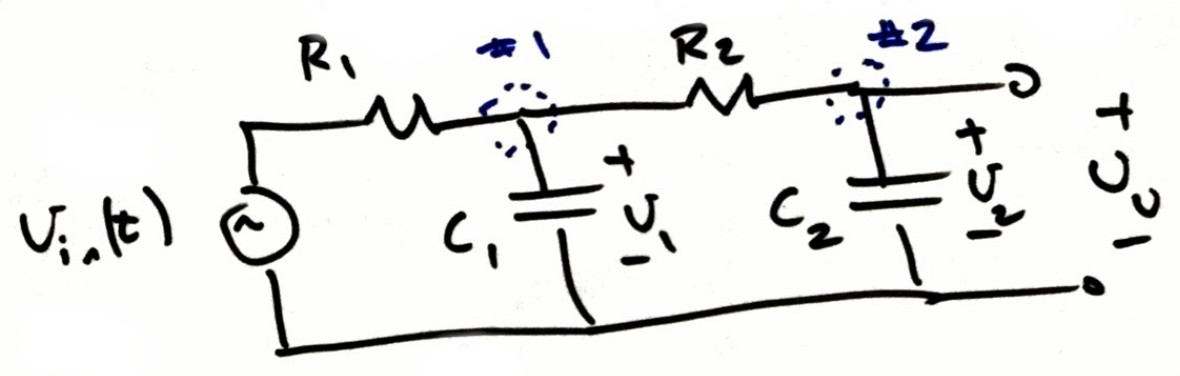
\includegraphics[width=1\linewidth]{figures/5/RCRC}
  \caption{Filter with two resistors and two capacitors.}
  \label{figure:lec5-RCRC}
\end{figure}
Perhaps a ``better'' filter could be constructed by using two capacitors and two resistors instead of just one.
\autoref{figure:lec5-RCRC} depicts the proposed circuit, which is a ``second-order circuit'' or ``second-order'' filter,
with values \(C_1 = C_2 = 1\unit{\(\mu\)F}\), \(R_1 = \frac{1}{3}\unit{M\(\Omega\)}\), and \(R_2 = \frac{1}{2}\unit{M\(\Omega\)}\).
KCL at the two dotted-circled upper nodes yields:
\begin{align}
  C_1 \dod{}{t} v_1 + \frac{v_1 - v_\text{in}(t)}{R_1} + \frac{v_1 - v_2}{R_2} &= 0\\
  C_2 \dod{}{t} v_2 + \frac{v_2 - v_1}{R_2} &= 0
\end{align}
In order to view this system of differential equations in state-space form, we will isolate derivatives on the LHS and emphasize that the RHS consists of linear combinations of \(v_1\), \(v_2\), and \(v_\text{in}(t)\):
\begin{align}
  \dod{}{t}v_1
  &= -v_1 \del{\del{\frac{1}{R_1} + \frac{1}{R_2}} \frac{1}{C_1}}
  + v_2 \del{\frac{ 1} {R_2C_1}} + v_\text{in}(t) \del{ \frac {1 }{R_1 C_1}}
  \\
  \dod{}{t} v_2
  &= v_1 \del{\frac1 {R_2 C_2}} - v_2 \del{\frac 1 {R_2 C_2}}
  \intertext{
  Written in matrix-vector form with physical parameters substituted,
  }
  \dod{}{t}
  \begin{bmatrix}
    v_1\\v_2
  \end{bmatrix}
  &=
  \begin{bmatrix}
    -5 & 2\\
    2 & -2
  \end{bmatrix}
  \begin{bmatrix}
    v_1\\v_2
  \end{bmatrix}
  % TODO use units
  +
  \begin{bmatrix}
    3\\0
  \end{bmatrix}
  v_\text{in}(t)
  \label{eq:lec5-RCRC-numerical}
\end{align}

\section{General state-space linear ODEs}
Generally, a system of linear differential equations similar to the one derived above has the following form:
\begin{align}
  \dod{}{t} \vec{x}
  &= A \vec{x} + \vec{b} u(t),
\end{align}
where \(\vec{x}\) is a vector and \(A\) is a \(2\times2\) matrix.

Suppose that \(A\) has an eigenvector \(\vec{v}\) for an eigenvalue \(\lambda\).
We propose the following solution to the homogeneous problem \(\od{}{t} \vec{x} = A \vec{x}\):
\begin{align}
  \vec{x} (t) = \vec{v} e^{\lambda t}
  \intertext{and verify that ``\(\od{}{t} \vec{x}\)'' and ``\(A \vec{x}\)'' for this candidate solution are equal:}
  \dod{}{t} \del{\vec{v} e^{\lambda t}}
  &= \lambda \vec{v} e^{\lambda t}\\
  A \del{\vec{v} e^{\lambda t}}
  &= \lambda \vec{v} e^{\lambda t}
\end{align}

\subsection{Detour: diagonalization of \(A\)}
Let's additionally assume that \(A\) has two linearly independent eigenvectors:
\begin{align}
  A \vec{v}_1 &= \lambda_1 \vec{v}_1 \\
  A \vec{v}_2 &= \lambda_2 \vec{v}_2
  \intertext{
  These two relationships can be expressed simultaneously using matrices that consolidate the eigenvectors (side by side) and eigenvalues (on a diagonal):
  }
  A
  \begin{bmatrix}
    \vec{v}_1 & \vec{v}_2
  \end{bmatrix}
  &=
  \begin{bmatrix}
    \vec{v}_1 & \vec{v}_2
  \end{bmatrix}
  \begin{bmatrix}
    \lambda_1 & 0 \\
    0 & \lambda _2
  \end{bmatrix}
  \intertext{Calling the former two matrices \(V\) and the latter \(\Lambda\),}
  AV &= V\Lambda
  \intertext{Because we chose two linearly independent eigenvectors to constitute \(V\), \(V\) is invertible.
  Stating \(A\) in terms of its eigenvectors and eigenvalues is called the \emph{eigenvector-eigenvalue decomposition} of \(A\):}
  A &= V \Lambda V^{-1}
\end{align}

\subsection{Second-order homogeneous solution from modes}
Generally, \(\vec{x}(0)\) will be a linear combination of \(\vec{v}_1\) and \(\vec{v}_2\):
\begin{align}
  \vec{x}(0)
  &= \tilde{x}_1(0) \vec{v}_1 + \tilde{x}_2(0) \vec{v}_2
  \label{eq:lec5-modal-decomp-IC}
  \intertext{These coefficients can be solved by inverting \(V\):}
  \begin{bmatrix}
    \tilde{x}_1 (0)\\
    \tilde{x}_2 (0)
  \end{bmatrix}
  &= V^{-1} \vec{x}(0)
  \intertext{We can build a homogeneous solution for \(\vec{x}(t)\) by superposing one-dimensional solutions in each eigenvector's respective direction:}
  \vec{x}(t)
  &= \vec{v}_1 e^{\lambda_1 t} \tilde{x}_1 (0)
  + \vec{v}_2 e^{\lambda_2 t} \tilde{x}_2 (0)\\
  &= V
  \begin{bmatrix}
    e^{\lambda_1 t} & 0\\
    0 & e^{\lambda_2 t}
  \end{bmatrix}
  \begin{bmatrix}
    \tilde{x}_1(0)\\
    \tilde{x}_2(0)
  \end{bmatrix}
  \intertext{To verify the initial condition, we can observe that the diagonal matrix of exponentials becomes an identity matrix at time \(0\):}
  \vec{x}(0) &=
  \begin{bmatrix}
    \vec{v}_1 & \vec{v}_2
  \end{bmatrix}
  \begin{bmatrix}
    1 & 0\\
    0 &1
  \end{bmatrix}
  \begin{bmatrix}
    \tilde{x}_1(0)\\
    \tilde{x}_2(0)
  \end{bmatrix},
\end{align}
which is true by construction (\autoref{eq:lec5-modal-decomp-IC}).

\subsection{Modal decomposition}
\begin{figure}
  \centering
  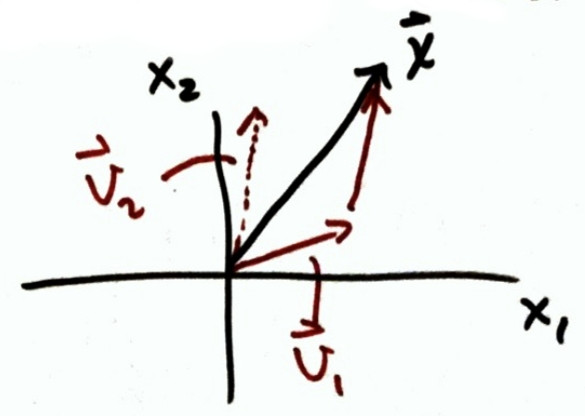
\includegraphics[width=0.5\linewidth]{figures/5/modal-synthesis}
  \caption{Decomposition of \(\vec{x}\) along eigenbasis directions \(\vec{v}_1\) and \(\vec{v}_2\).}
  \label{figure:lec5-modal-synthesis}
\end{figure}
In the previous section, we wrote \(\vec{x}(0)\) in eigenbasis-aligned coordinates \(\tilde{x}_1(0)\) and \(\tilde{x}_2(0)\).
In this section, we will follow \(\tilde{x}_1\) and \(\tilde{x}_2\) as functions of \(t\).
Recall that the eigenbasis-aligned coordinates are defined as follows:
\begin{align}
  \vec{x} &=
  \begin{bmatrix}
    \vec{v}_1 & \vec{v}_2
  \end{bmatrix}
  \begin{bmatrix}
    \tilde{x}_1 \\ \tilde{x}_2
  \end{bmatrix}
  = V \vec{\tilde x}.
  \intertext{In reverse,}
  \vec{\tilde x}
  &= V^{-1} \vec{x}.
  \intertext{We can use the Chain Rule to obtain a differential equation for \(\vec{\tilde x}\):}
  \dod{}{t} \vec{\tilde x}
  &= V^{-1} \dod{}{t} x\\
  &= V^{-1} \del{A \vec{x} + \vec{b} u}\\
  &= V^{-1} A V \vec{\tilde x} + V^{-1} \vec{b} u \\
  &=
  \begin{bmatrix}
    \lambda_1 & 0 \\
    0 & \lambda_2
  \end{bmatrix} \vec{\tilde x}
  + \vec{\tilde b} u, \quad \vec{\tilde b} = V^{-1} b
\end{align}
This vector differential equation is effectively scalar in each variable, in which scalar techniques can be applied separately.
The separation of \(x\) into its eigenbasis-aligned components is called \emph{modal decomposition};
\( \vec v_1 e^{\lambda_1 t}\) and
\( \vec v_2 e^{\lambda_2 t}\) are the two \emph{modes} of this system.

\chapter{Diagonalization to solve vector differential equations}
In the last lecture, a second-order low-pass filter circuit using two resistors and two capacitors led us to the following differential equation:
\begin{align}
  \dod{}{t} \vec{x}
  &= A \vec{x} + \vec{b} u,
\end{align}
where \(\vec{x} = \begin{bmatrix}
  v_1(t) \\ v_2(t)
\end{bmatrix}\)
and \(\vec{x}(0)\) or \(\vec{x}(t_0)\) is known.
We represented \(\vec{x}\) as a linear combination of \(A\)'s eigenvectors \(\vec{v}_1\) (for eigenvalue \(\lambda_1\)) and \(\vec{v}_2\) (for eigenvalue \(\lambda_2\)):
\begin{align}
  \vec{x}
  &= \vec v_1 \tilde x_1
  + \vec v_2 \tilde x_2\\
  &=
  \begin{bmatrix}
    \vec v_1 & \vec v_2
  \end{bmatrix}
  \begin{bmatrix}
    \tilde x_1\\
    \tilde x_2
  \end{bmatrix}
    = V \vec {\tilde x}
\end{align}
We will assume that \(\lambda_1\) and \(\lambda_2\) are distinct, which implies that \(A\) has an invertible matrix of linearly independent eigenvectors \(V\).%
% \footnote{The proof of this fact is beyond the scope of this course.}
 We established that
\begin{align}
  A V &= V \Lambda, \quad
  V = \begin{bmatrix}
    \vec v_1 & \vec v_2
\end{bmatrix}, \quad
  \Lambda = \begin{bmatrix}
    \lambda_1 & 0 \\
    0 & \lambda 2
\end{bmatrix}.
\end{align}
These findings are summarized in \autoref{figure:lec6-diagonalization-commutative}, which shows how \(\vec x\), \(A \vec{x}\), \(\vec {\tilde x}\), and \(\Lambda \vec{\tilde x}\) are related by matrix multiplication (along arrows).

\begin{figure}
  \centering
  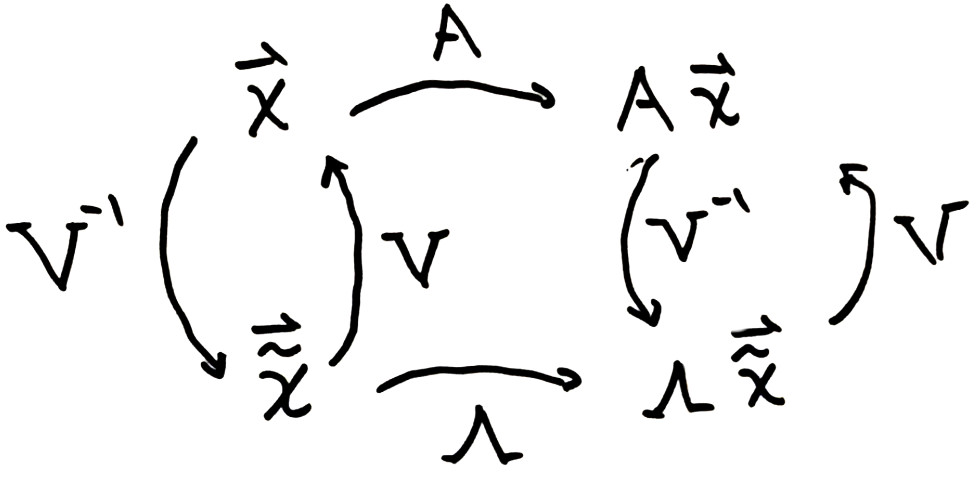
\includegraphics[width=0.75\linewidth]{figures/6/diagonalization-commutative}
  \caption{Illustration of multiplication actions of \(A\), \(\Lambda\), \(V\), and \(V^{-1}\).}
  \label{figure:lec6-diagonalization-commutative}
\end{figure}

\section{Solution technique}
A system
\begin{align}
  \dod{}{t} \vec x
  &= A \vec x + \vec b u; \quad \vec x (t_0)
\end{align}
is solved as follows:
\begin{enumerate}
  \item Compute eigenvalues \(\lambda_1\) and \(\lambda_2\) of \(A\), as well as their respective eigenvectors \(\vec v_1\) and \(\vec v_2\).
  \item Construct \(V = \begin{bmatrix}
            \vec v_1 & \vec v_2
        \end{bmatrix}\)
        and define
        \(\vec{\tilde x} = V^{-1} x\).
  \item
  Construct \(\Lambda = \begin{bmatrix}
    \lambda_1 & 0 \\
    0 & \lambda_2
  \end{bmatrix}\) and \(\tilde b = V^{-1} b\).
  Solve the differential equation
  \(\dod{}{t} \vec{\tilde x} = \Lambda \vec{\tilde x} + \tilde b u\)
  with initial condition \(\tilde x(t_0) = V^{-1} x(t_0)\). (More on this later.)
  \item Recover a solution for \(\vec x\) using \(\vec x = V \vec{\tilde x}\).
\end{enumerate}

\section{Numerical example from RCRC circuit}
\autoref{eq:lec5-RCRC-numerical} captured a second-order low-pass filter using
\begin{align}
  A = \begin{bmatrix}
    -5 & 2 \\ 2 & -2
\end{bmatrix} \quad \text{and} \quad
  \vec b = \begin{bmatrix}
    3 \\ 0
\end{bmatrix}.
\end{align}
We will solve the differential equation for \(\vec x = \begin{bmatrix}
  v_1 \\ v_2
\end{bmatrix}\) using the technique of the previous section.

\subsection{Eigenvalues and eigenvectors}
We will solve for eigenvectors \(\lambda\) as roots of \(\det\del{\lambda I - A}\), the characteristic polynomial of \(A\).
\begin{align}
  \det
  \begin{bmatrix}
    \lambda + 5 & -2 \\
    -2 & \lambda + 2
  \end{bmatrix}
  &= \lambda^2 + 7\lambda + 6 = 0\\
  \intertext{This quadratic equation in the indeterminate \(\lambda\) is called the \emph{characteristic equation} of \(A\).
  It has the following roots:}
  \lambda_1 &= -1; \quad \lambda_2 = -6.
  \intertext{Next we will solve for an eigenvector belonging to eigenvalue \(\lambda_1\), by choosing a nonzero vector from the null space of \(\lambda_1I - A\):}
  \lambda_1 I - A &= \begin{bmatrix}
    4 & -2 \\
    -2 & 1
  \end{bmatrix}\\
  \vec v_1 &= \begin{bmatrix}
    1 \\ 2
  \end{bmatrix}
  \intertext{\ldots and, \emph{mutatis mutandis}, for \(\lambda_2\):}
  \lambda_2 I - A &= \begin{bmatrix}
    -1 & -2 \\
    -2 & -4
  \end{bmatrix}\\
  \vec v_2 &= \begin{bmatrix}
    2 \\ -1
  \end{bmatrix}
\end{align}

\subsection{Differential equation in new coordinates}
In our example,
\begin{align}
  V &= \begin{bmatrix}
    1 & 2 \\
    2 & -1
\end{bmatrix}, \quad \text{so}\\
V^{-1} &= \begin{bmatrix}
  \frac{1}{5} & \frac{2}{5} \\
  \frac{2}{5} & -\frac{1}{5}
\end{bmatrix}.
\intertext{
Our differential equation in \(\vec{\tilde x}\) will be
}
\dod{}{t} \vec{\tilde x}
&= \Lambda \vec{\tilde x} + V^{-1} \vec b u\\
&= \begin{bmatrix}
  -1 & 0 \\
  0 & -6
\end{bmatrix}
\vec{\tilde x}
+ \begin{bmatrix}
  \frac{3}{5} \\ \frac{6}{5}
\end{bmatrix}.
\intertext{
   With \(t_0 = 0\), \(\vec {\tilde x}\) is solved as follows:
}
\vec{\tilde x} (t)
&= \del{\text{homogeneous solution}} + \del{\text{particular solution}}\\
&= \begin{bmatrix}
  e^{\lambda_1 t} & 0\\
  0 & e^{\lambda_2 t}
\end{bmatrix}
\vec{\tilde x} (0)
+ \int_{0}^t
\begin{bmatrix}
  e^{\lambda_1(t - \tau)} & 0 \\
  0 & e^{\lambda_2(t - \tau)}
\end{bmatrix}
\vec{\tilde b}
u(\tau)
\dif \tau,
\end{align}
viz., in individual components,
\begin{align}
  \begin{cases}
  \tilde x_1 (t)
  = e^{\lambda_1 t} \tilde x_1(0) + \int_{0}^t e^{\lambda_1(t - \tau)}
    \tilde b_1 u(\tau) \dif \tau\\
  \tilde x_2 (t)
  = e^{\lambda_2 t} \tilde x_2(0) + \int_{0}^t e^{\lambda_2(t - \tau)}
    \tilde b_2 u(\tau) \dif \tau
\end{cases}
\end{align}

\subsection{Solution in original coordinates}
A solution for \(\vec x(t)\) may be reconstituted from eigenbasis-aligned coordinates using the following equation:
\begin{align}
  \vec x(t)
  &= \begin{bmatrix}
    \vec v_1 & \vec v_2
\end{bmatrix}
\begin{bmatrix}
  \tilde x_1 (t) \\
  \tilde x_2 (t)
\end{bmatrix}.
\end{align}

\section{Introduction to inductors}
\begin{figure}
  \centering
  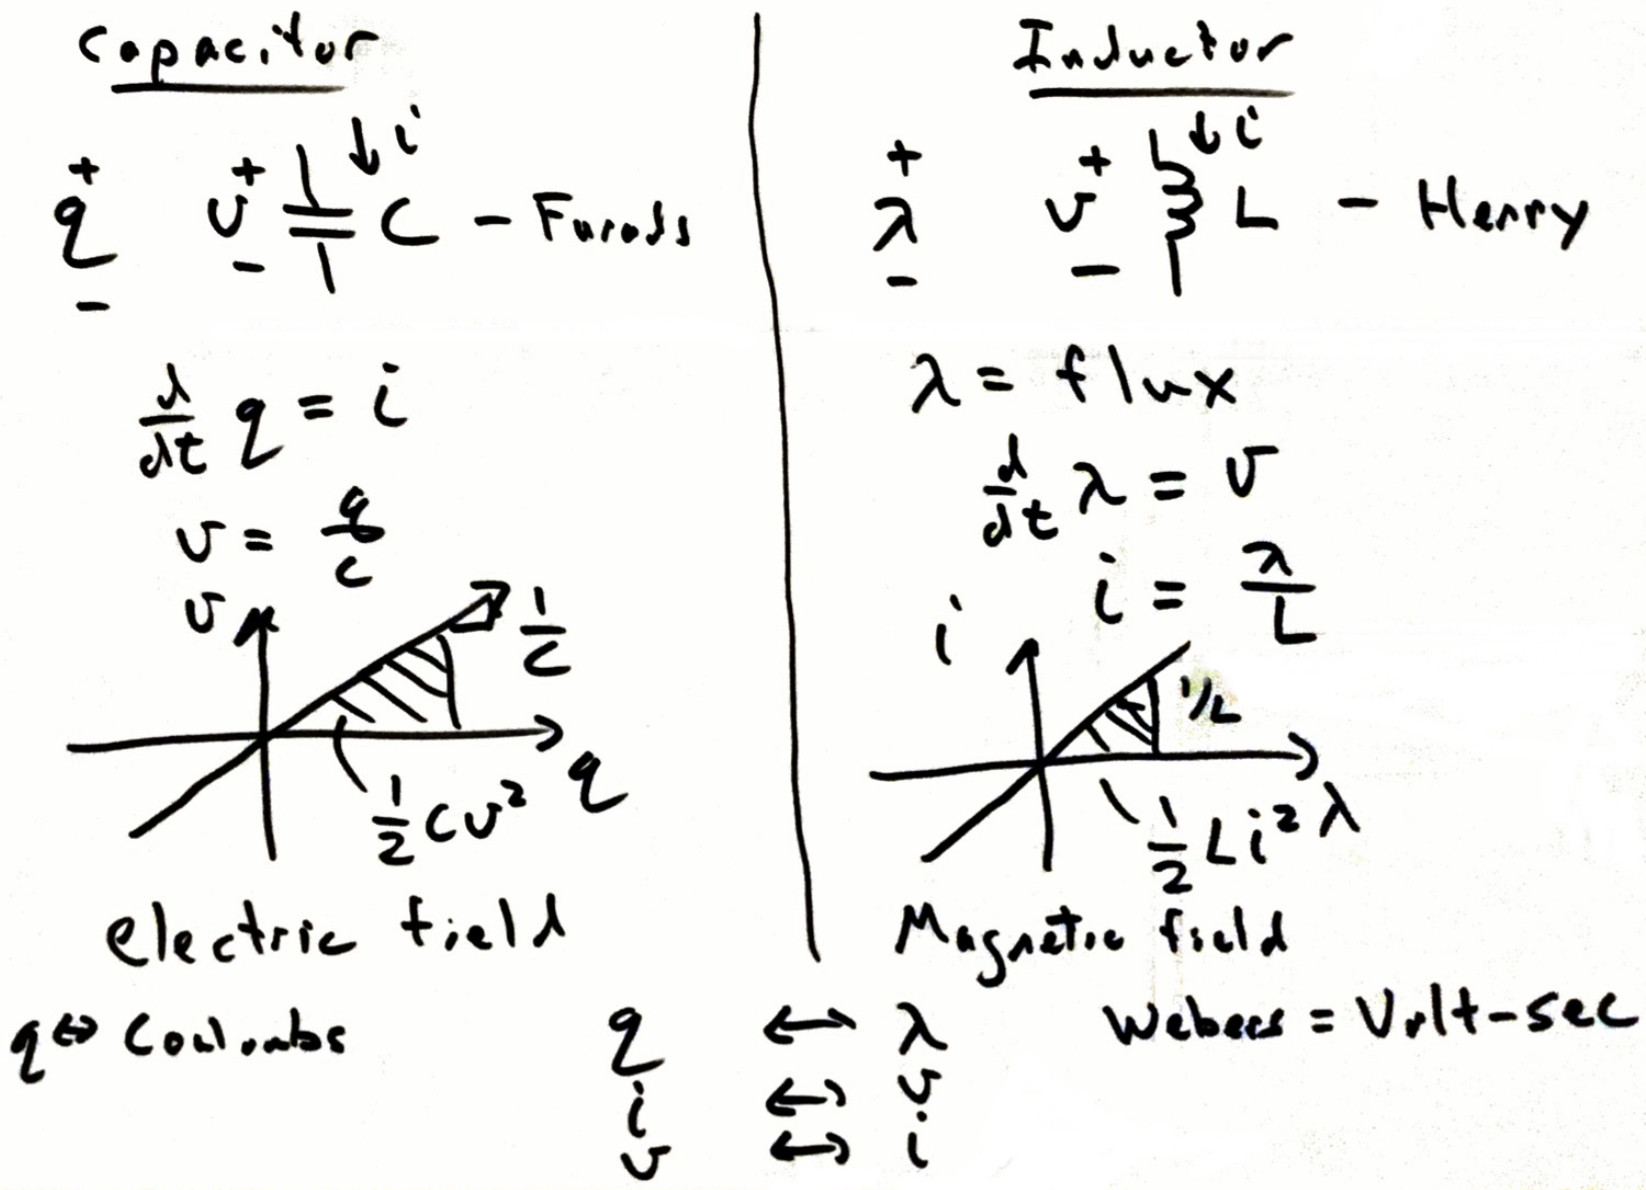
\includegraphics[width=1\linewidth]{figures/6/cap-vs-ind}
  \caption{Parallels between capacitors and inductors.}
  \label{figure:lec6-cap-vs-ind}
\end{figure}
Inductors are a branch element that are analogous to capacitors.
\autoref{figure:lec6-cap-vs-ind} compares them with capacitors,
and the parallels are repeated below.
\begin{align}
  q &= \text{charge (Coulomb)}
  & \lambda &= \text{flux (Weber = Volt-second)}\\
  \dod{}{t} q &= i & \dod{}{t} \lambda &= v\\
  v &= \frac{q}{C} & i &= \frac{\lambda}{L} \\
  E_{C} &= \frac{1}{2} Cv^2 & E_{L} &= \frac{1}{2} Li^2
\end{align}

\section{Example: RL circuit}
\begin{figure}
  \centering
  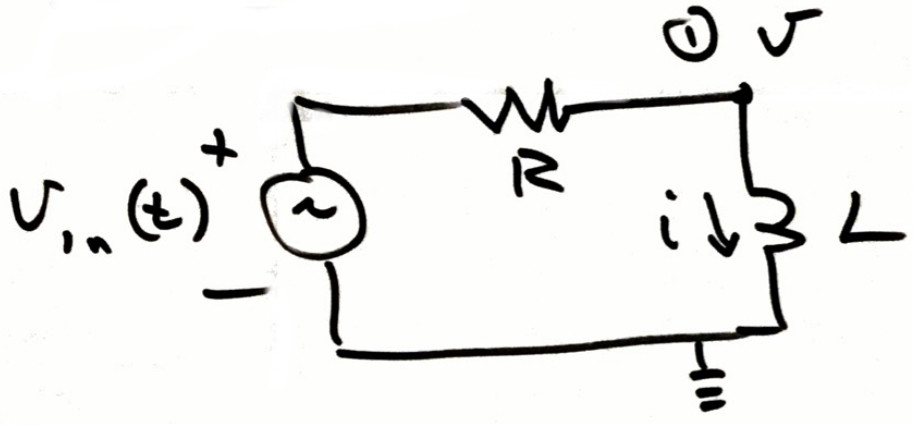
\includegraphics[width=0.75\linewidth]{figures/6/RL}
  \caption{RL circuit, which is similar to an RC circuit (cf.~\autoref{figure:lec4-RC}).}
  \label{figure:lec6-RL}
\end{figure}
\autoref{figure:lec6-RL}
shows a circuit with a time-varying voltage source, a resistor, and an inductor.
KCL at the marked upper right node yields
\begin{align}
  \frac{v - v_\text{in}}{R} + i &= 0.
  \intertext{In addition, from the current-voltage relationship of an inductor,}
  L \dod{}{t} i &= v.
  \intertext{Eliminating \(v\) and isolating \(\dod{}{t} i\), we have}
  \dod{}{t}i &= -\frac{R}{L} i + \frac{v_\text{in}}{L}.
\end{align}
The state variable for an inductor is \(i\), and this differential equation may be solved the same way we solved RC circuits.

\end{document}
